%============================================================
%  CS 495 Capstone Research Report
%  Binomial Option Pricing in Practice:
%  Using CRR American Option Valuation to Detect Mispricing
%  and Inform a Profit-Maximizing Trade Strategy on AMD
%  Calls and Puts
%============================================================

\documentclass[12pt, letterpaper]{article}

%------------------------------------------------------------
%  PACKAGES
%------------------------------------------------------------
\usepackage[margin=1in]{geometry}
\usepackage{setspace}
\doublespacing

\usepackage{times}              % Times New Roman font

\usepackage{amsmath, amssymb}   % Math environments and symbols

%  natbib  — provides \citet, \citep, \citeauthor, \citeyear
%  round   — parentheses around year; authoryear — Author-Year style
%  DO NOT load apacite alongside natbib; they conflict.
\usepackage[authoryear, round]{natbib}

\usepackage{hyperref}           % Clickable DOIs and URLs
\hypersetup{
    colorlinks = true,
    linkcolor  = black,
    urlcolor   = blue,
    citecolor  = black
}

\usepackage{graphicx}           % \includegraphics for figures
\graphicspath{{./}{../../assets/figures/}{../../slides/figures/}{../../project/outputs/}}
\usepackage{booktabs}           % Professional table rules
\usepackage{array}
\usepackage{parskip}
\setlength{\parindent}{0.5in}
\usepackage{indentfirst}

%------------------------------------------------------------
%  PAGE BREAK BEFORE EVERY TOP-LEVEL SECTION
%  Redefine \section to issue \clearpage first so each
%  \section{...} starts on a fresh page. Optional arguments
%  (\section[Short]{Long}) still work because the original
%  \section is invoked after the page break.
%------------------------------------------------------------
\let\oldsection\section
\renewcommand{\section}{\clearpage\oldsection}

%------------------------------------------------------------
%  PAGE BREAK BEFORE EVERY SUBSECTION EXCEPT X.1
%  Every \subsection{...} starts on a fresh page UNLESS it is
%  the first subsection of its parent section (i.e., X.1).
%  Mechanism: \section resets the subsection counter to 0;
%  if the counter is still 0 when \subsection fires, this is
%  X.1 and no page break is issued. If the counter is > 0,
%  we are about to render X.2 or later and \clearpage runs.
%------------------------------------------------------------
\let\oldsubsection\subsection
\renewcommand{\subsection}{%
  \ifnum\value{subsection}>0 \clearpage\fi
  \oldsubsection
}

%------------------------------------------------------------
%  TITLE BLOCK
%------------------------------------------------------------
\title{
  \large CS495 Capstone Research Report \\[6pt]
  Mathematical and Empirical Models in Agreement:\\
  Cross-Validating CRR Binomial Pricing and Machine Learning\\
  for Crowd Mispricing Detection in Equity Options\\[6pt]
}
\author{DeWayne Dantzler \\[4pt] CS 495 Capstone Project 6}
\date{May 2026}

%============================================================
\begin{document}

\maketitle
\thispagestyle{empty}
\newpage

%------------------------------------------------------------
\tableofcontents
\newpage

%============================================================
%  SECTION 1 — INTRODUCTION
%============================================================
\section{Introduction}

\subsection{Background and Context}

Options markets represent one of the most sophisticated and
consequential arenas in modern financial markets, with daily notional
volumes exceeding trillions of dollars across U.S.\ equity exchanges.
At their core, options contracts are instruments of risk transfer:
they grant the holder the right, but not the obligation, to buy or
sell an underlying asset at a predetermined price---the strike---on or
before a specified expiration date. The premium charged for this right
encodes the collective market belief about future price uncertainty,
making options markets functionally analogous to prediction markets in
which crowd sentiment drives prices away from theoretical fair value.

The mathematical foundation for rational options pricing was
established in two landmark papers. \citet{BlackScholes1973} derived a
closed-form continuous-time formula for European option valuation under
the assumption of constant volatility and no early exercise. Shortly
thereafter, \citet{Cox1979} introduced the Cox--Ross--Rubinstein (CRR)
binomial lattice, a discrete-time framework that replicates the
Black--Scholes result in the limit while adding two critical
capabilities: native handling of American-style early exercise and
accommodation of discrete dividend payments. These two contributions
remain the twin pillars of options pricing in both academic instruction
and practitioner workflows.

\newpage
Despite the elegance of these theoretical frameworks, a persistent gap
exists between the prices that models produce and the premiums that
markets charge. Behavioral forces---herding around round strikes,
implied volatility overpricing driven by fear, and systematic skew in
out-of-the-money puts---distort market prices in predictable ways.
This gap between theoretical fair value and observed market premium is
not merely academic: it is potentially exploitable by a disciplined,
model-driven strategy. The present project addresses exactly this gap,
applying the CRR binomial model to live Advanced Micro Devices, Inc.\
(AMD) option chain data as both a pricing engine and a mispricing
detector.

A second, less examined gap motivates this project alongside the
classical mispricing question. The empirical literature on options
mispricing has historically treated mathematical no-arbitrage pricing
and statistical or machine-learning approaches as \emph{alternatives}:
either one is used to bound the other, or they are evaluated head to
head on a common pricing-error metric \citep{Carr2009, Jackwerth1996}.
What the literature has not done is treat the two as
\emph{independent voters} on the same mispricing question, asked from
disjoint inputs, and use their agreement (or disagreement) as the
diagnostic. The mathematical price relies on a no-arbitrage lattice
calibrated to realized historical volatility; a well-designed
machine-learning price can be trained on binary outcome labels with
implied volatility deliberately excluded. When two such models, sharing
neither inputs nor training data, agree that a given contract is
mispriced, that agreement is a far stronger signal than either model
alone could provide. The present project operationalizes this
cross-validation framework and is, to the author's knowledge, the first
to do so for retail-accessible options data with a regime-conditioned
position-sizing layer.

\subsection{Problem Statement}

The central problem this project addresses is the following: when an
options pricing model produces a theoretical fair value that diverges
from the observed market premium, is that divergence large enough, and
reliable enough, to justify a trade? If so, how much of the available
capital should be committed, given the inherent uncertainty of the
model?

This problem is operationalized using a live AMD option chain captured
from the Fidelity trading platform in April 2026, with AMD trading at
approximately \$275.10 and a May 8, 2026 expiration date. Four
specific trade tickets are examined: Sell Call \$277.50 (limit
\$14.25), Buy Put \$280 (limit \$18.55), Buy Call \$280 (limit
\$14.20), and Sell Put \$280 (limit \$17.87). The implied volatility on
the AMD chain ranges from approximately 64\% to 65\%---a level that
raises immediate questions about whether the crowd is overpricing
uncertainty relative to what the historical realized volatility would
justify.

The problem is compounded by the American-style nature of all four
contracts. Unlike European options, American options may be exercised
at any time before expiration, a feature that the closed-form
Black--Scholes model cannot handle. The CRR binomial lattice, through
its backward-induction algorithm, is uniquely suited to determine not
only the fair value of these contracts but also the critical stock
price below which early exercise of the AMD put options becomes
optimal.

A further problem lies one level above the pricing question itself: a
single-model edge signal cannot self-certify. When a no-arbitrage
pricer flags a contract as overpriced, the analyst has no purely
internal check against the possibility that the divergence is a model
artifact---a no-dividend assumption, a volatility input estimated from
a noisy realized window, a microstructure cost the model omits, or a
regime mismatch between the calibration sample and the live chain.
The meta-problem this project addresses is therefore not only ``is
this contract mispriced?'' but ``is the detected mispricing real or a
model artifact?'' The proposed answer is cross-validation between two
fully independent pricing approaches---a mathematical, no-arbitrage
CRR engine and an empirical, IV-free machine-learning classifier
trained on realized binary outcomes. Agreement between the two on the
direction of the mispricing constitutes the diagnostic that the signal
is structural rather than artifactual; disagreement zones become
findings in their own right by isolating regimes in which one model
captures information the other misses.

\subsection{Purpose and Objectives}

The purpose of this project is to implement a CRR American binomial
option pricer in Python, validate it against observed AMD market
premiums and platform-reported Greeks, and use the pricing output as
the probability estimator in a Kelly Criterion trade-sizing framework.
Beyond this single-model pricing pipeline, the project implements an
independent machine-learning probability estimator (Layer~2) and
operationalizes a cross-validation framework in which the two
models---one mathematical, one empirical---are evaluated as
independent voters on the same mispricing question. The full
three-layer pipeline is then evaluated out-of-sample through a
chronological walk-forward backtest. The specific objectives are:

\begin{enumerate}
  \item Implement the CRR American binomial lattice (no dividends) in
        vectorized Python and price all four AMD trade tickets at
        $N = 100$ steps.
  \item Validate pricing accuracy against observed market premiums,
        targeting a percentage error within $\pm 5\%$ for all four
        contracts.
  \item Compute the five standard option Greeks---Delta ($\Delta$),
        Gamma ($\Gamma$), Theta ($\theta$), Vega ($\nu$), and Rho
        ($\rho$)---via centered finite differences and validate them
        against the Greek values reported on the AMD Fidelity trade
        tickets.
  \item Identify the early exercise boundary for the AMD American put
        options: the critical stock price $S^{*}$ below which early
        exercise dominates continuation.
  \item Compute the mispricing edge for each contract as the signed
        percentage deviation between the model price and the observed
        market premium, and apply the Kelly Criterion to derive
        optimal position-sizing recommendations.
  \item Assess the robustness of both pricing and Kelly fractions
        through sensitivity analysis across implied volatility, the
        risk-free rate, and time to expiration.
  \item Train an independent Layer~2 ITM/OTM probability estimator
        using XGBoost on the AAPL 2016--2020 options dataset, with
        implied volatility deliberately excluded from the feature set
        and the binary expiration outcome as the supervision signal,
        so the resulting probability estimate is structurally
        independent of the CRR price.
  \item Cross-validate the Layer~1 (mathematical) and Layer~2
        (empirical) edge signals on a shared sample of $3{,}000$ AAPL
        contracts, conditioning on the crowd-bias regime classifier,
        and test the null hypothesis that the two layers are no more
        in agreement than chance would predict.
  \item Walk-forward backtest the integrated Layer-1 + Layer-2 +
        Layer-3 pipeline across the AAPL 2017--2021 chronological
        chain ($57{,}231$ trade decisions), with regime-conditioned
        Kelly position sizing, and evaluate whether the
        cross-validated signal translates into positive out-of-sample
        expected value.
\end{enumerate}

\subsection{Significance}

This research is significant on four levels.

The primary contribution is methodological: the project is, to the
author's knowledge, the first to cross-validate a no-arbitrage
mathematical option pricer against an independently trained empirical
machine-learning classifier on a shared options sample, conditioned on
a behavioral regime detector. Prior work in options mispricing has
treated mathematical and statistical approaches as competing pricers
to be benchmarked against each other on pricing error, not as
independent voters on the same mispricing question. The
implementation enforces structural independence: the Layer~1 (CRR)
price is calibrated to 30-day realized volatility and uses no market
premium as input; the Layer~2 (XGBoost) classifier is trained on
binary in-the-money expiration outcomes and explicitly excludes
implied volatility from its feature set. When two such models, sharing
neither inputs nor training data, agree that a given contract is
mispriced under the same regime classifier, that agreement is
diagnostic evidence that the mispricing reflects a structural property
of the market rather than an artifact of either model. The
regime-conditional Pearson correlation of $r = 0.413$
($p = 2.4 \times 10^{-10}$, $n = 217$) reported in
Section~\ref{sec:cross_model} is the central empirical instantiation
of this contribution.

XGBoost \citep{Chen2016} was selected as the Layer~2 estimator for
four reasons specific to the cross-validation use case. First, it
natively handles the mixed scale of options-market features---moneyness
ratios, days to expiration, realized-vs-implied volatility spreads,
volume-to-open-interest ratios, and dollar bid-ask spreads---without
the imputation or feature-scaling pipeline a logistic regression or
neural network would require. Second, its tree-ensemble structure
captures non-linear feature interactions (e.g., the moneyness $\times$
DTE interaction that drives ITM probability for short-dated puts)
without an explicit interaction-term specification. Third, it
performs strongly on the moderate-sized labeled samples typical of
single-underlying options-chain data, where deep neural networks tend
to overfit and parametric models tend to misspecify. Fourth, its
probabilistic outputs are amenable to Platt-style calibration and
yield a Brier score below the naïve baseline, which is the metric the
cross-validation framework requires from a probability estimator. The
training procedure---walk-forward 60/20/20 split on AAPL 2016--2020
chain data, binary ITM/OTM labels at expiration, no lookahead bias,
and feature exclusion of implied volatility---is detailed in
Section~\ref{sec:worked_example} and Section~\ref{sec:cross_model}.

Beyond the cross-validation contribution, this research bridges the
gap between academic option pricing theory and the live trading
interfaces that practitioners interact with daily. Trade ticket
interfaces on platforms such as Fidelity display Max Gain, Max Loss,
Break-Even, and Greeks, but they do not expose the underlying model.
Reconstructing these values from the CRR binomial lattice makes the
pricing mechanism transparent and auditable, and the open-source
Streamlit calculator distributed with this project lets a retail
trader run the same diagnostic on any contract of interest.

The project also operationalizes the prediction-market analogy for
options pricing. Just as prediction markets reflect behavioral biases
that a calibrated model can detect \citep{Wolfers2004}, the AMD
options chain and the AAPL backtest sample both reflect the crowd's
collective overestimate of future volatility. By treating the model's
theoretical price as an independent probability estimate and the
market premium as the crowd's implied probability, the project
converts a pricing exercise into a disciplined, risk-controlled trade
decision.

Finally, the financial stakes of accurate pricing are non-trivial. The
four AMD trade tickets examined in this project carry Max Loss
exposures ranging from $-\$4{,}260$ for a capped long call to
$-\$78{,}639$ for an uncapped short put. The Kelly Criterion framework
ensures that position sizing is proportional to the model's confidence
in the detected mispricing, providing a formal mechanism for risk
management under model uncertainty \citep{MacLean2010}. The
persistence of the IV-RV spread as a detectable edge is consistent
with documented anomalies in the efficient market literature
\citep{Fama1970}---specifically the volatility risk premium that
options markets systematically embed above and beyond what realized
historical volatility would justify \citep{Carr2009}.

\subsection{Cross-Model Validation Framework}
\label{sec:cv_framework}

The cross-model validation framework formalizes how the two pricing
layers are forced to behave as independent voters on the same
mispricing question. This subsection states the framework, summarizes
the Layer-2 training procedure and rationale for the XGBoost choice,
defines the regime-conditional null hypothesis the framework tests,
and enumerates the three formal research hypotheses (H1, H2, H3) that
structure the Results section.

\paragraph{Independence requirement.} The framework's diagnostic
power depends entirely on the structural independence of the two
layers. Layer~1 (CRR) accepts the underlying price $S_{0}$, strike
$K$, time to expiration $T$, risk-free rate $r$, and a volatility
input $\sigma$, and produces a no-arbitrage fair value
$V_{\text{model}}$ through backward induction over the binomial
lattice. Critically, the volatility input in this project is the
30-day realized volatility ($\sigma = \sigma_{\text{RV30}}$), not the
implied volatility back-solved from the market premium. Calibrating
the lattice to implied volatility would produce $V_{\text{model}}
\equiv V_{\text{market}}$ by construction and reduce the Layer~1 edge
to identically zero. Layer~2 (XGBoost) accepts a feature vector
consisting of moneyness ratio $S/K$, days to expiration (DTE), the
realized-vs-implied volatility spread, the volume-to-open-interest
ratio, and the dollar bid-ask spread. The market premium and the
implied volatility are both excluded from the Layer~2 feature set.
The Layer~2 output is an independent ITM probability estimate
$\hat{p}_{\text{indep}}$ that, compared against the market-implied
probability $\hat{q}_{\text{market}}$, produces the Layer~2 edge.
Neither layer is given access to the other's input or output during
prediction, and neither is trained on labels derived from the other.

\paragraph{XGBoost training procedure.} The Layer-2 classifier is
trained on the AAPL options chain dataset for 2016--2020
($\sim 101{,}535$ contracts), using the binary in-the-money expiration
outcome as the supervision signal: a contract is labeled $1$ if it
expired ITM and $0$ otherwise. The data are partitioned chronologically
into a 60\% training window, a 20\% validation window for
hyperparameter selection and early stopping, and a 20\% held-out
test window, ensuring zero lookahead bias. Separate models are trained
for puts and calls because the conditional ITM probability surface
differs in shape between the two contract types. The output
probabilities are calibrated using Platt scaling on the validation
window. Model selection is performed on the validation Brier score,
which the chosen XGBoost configuration drives below the $0.25$ naïve
baseline. The cross-validation sample of $3{,}000$ contracts used in
Section~\ref{sec:cross_model} is drawn exclusively from the held-out
test window so that the Layer-1 and Layer-2 outputs are out-of-sample
for both models.

\paragraph{Why XGBoost.} The choice of XGBoost over a simpler
baseline (logistic regression, random forest) or a more complex one
(deep neural network) is driven by four considerations specific to
this cross-validation use case. First, the feature set is small,
heterogeneous in scale, and contains pre-known non-linear
interactions (moneyness $\times$ DTE for short-dated puts; bid-ask
spread $\times$ volume for liquidity-constrained contracts), all of
which gradient-boosted trees handle natively without feature
engineering. Second, the model must produce well-calibrated
probabilities (not merely good classification accuracy) because
$\hat{p}_{\text{indep}}$ enters a Kelly-fraction calculation
downstream; XGBoost's gradient-of-logloss objective combined with
Platt-scaled calibration achieves Brier $= 0.211$, comfortably below
the $0.25$ naïve baseline. Third, the moderate sample size and
tabular structure of options-chain data place this problem squarely in
the regime where gradient-boosted trees dominate deep neural networks
in the practitioner literature \citep{Grinsztajn2022}. Fourth, the
model must be robust enough to operate on regime-dependent feature
distributions; the tree-ensemble structure provides this robustness
without the regularization tuning a neural network would require.
Baseline logistic regression was evaluated and underperforms XGBoost
on both Brier score and ITM-rate-by-edge-zone agreement, confirming
that the non-linear interactions captured by the boosting layers are
load-bearing rather than incidental.

\paragraph{Regime-conditional null hypothesis.} The aggregate
correlation between the Layer-1 and Layer-2 edges across the full
$3{,}000$-contract sample is not the intended diagnostic. The
hypothesis the framework tests is regime-conditional: among contracts
labeled as drawn from the herding regime by the IV/RV-30 classifier
(Section~\ref{sec:regime}), do Layer-1 and Layer-2 edges correlate
significantly more strongly than across the full sample? The null
hypothesis is $H_{0}: r_{\text{herding}} = r_{\text{pooled}}$; the
alternative is $H_{1}: r_{\text{herding}} > r_{\text{pooled}}$. The
test is two-sample on Fisher-transformed correlation coefficients
with the pooled $r$ as the reference. Confirmation of the alternative
would be empirical evidence for Samuelson macro-inefficiency
\citep{Fama1970}: markets are micro-efficient in aggregate but
behaviorally biased in identifiable regimes. The structure of the
aggregate-vs-conditional inversion is a textbook instance of
Simpson's Paradox: a pooled correlation of $r = 0.032$ that conceals
a regime-conditional correlation of $r = 0.413$ in the herding
subsample.

\paragraph{Research hypotheses.} The above framework structures three
formal hypotheses that the Results section evaluates:
\begin{description}
  \item[\textbf{H1 --- Pricing accuracy.}] The CRR American binomial
        lattice at $N = 100$ steps prices the four AMD trade tickets
        within $\pm 5\%$ of their observed market premiums. Evaluated
        in Section~\ref{sec:cv_h1}.
  \item[\textbf{H2 --- Numerical convergence.}] The CRR price for
        each AMD contract stabilizes well before the operating step
        count $N = 100$, with the log-residual against the asymptotic
        reference price crossing the \$0.01 threshold no later than
        $N \approx 100$. Evaluated in Section~\ref{sec:cv_h2}.
  \item[\textbf{H3 --- Cross-model agreement under herding.}] The
        regime-conditional Pearson correlation between the Layer-1
        and Layer-2 edges in the herding subsample is significantly
        greater than the pooled correlation, with the herding-subsample
        correlation testing as significantly different from zero at
        $\alpha = 0.01$. Evaluated in Section~\ref{sec:cross_model}
        and out-of-sample in the walk-forward backtest of
        Section~\ref{sec:backtest}.
\end{description}

%------------------------------------------------------------
\subsection{Scope and Boundaries}

This project is scoped as follows. All four AMD contracts are treated
as American-style options with backward-induction early exercise
evaluated at every node. No dividend adjustment is applied; the
standard CRR risk-neutral probability formula is used throughout:

\begin{equation}
  p \;=\; \frac{e^{r\,\Delta t} - d}{\,u - d\,}
  \label{eq:crr_prob}
\end{equation}

\noindent The analysis covers only vanilla calls and puts on a single
underlying (AMD) with a single expiration date (May 8, 2026). Exotic
derivatives, multi-asset portfolios, and European-equivalent
convergence experiments are excluded. The Kelly Criterion analysis is
strictly analytical; no real trades are executed.

\subsection{Report Outline}

The remainder of this report is organized as follows. Section~2
surveys the relevant literature, covering foundational and applied
papers on the CRR binomial model, American option early exercise,
options market mispricing, the prediction-market analogy, the
Kelly Criterion, and the efficient-market hypothesis. Section~3
describes the experimental methodology and model implementation,
including research design, data collection, preprocessing steps, the
analytical pipeline (Layer~1 CRR pricer, Layer~2 XGBoost classifier,
and Layer~3 cross-model comparison), a worked example carrying a
single contract through both pricing layers, evaluation metrics, and
tools. Section~4 presents the full results, organized to mirror the
three research hypotheses introduced in
Section~\ref{sec:cv_framework}: model performance and pricing
validation (H1), numerical convergence (H2), early exercise
boundary, mispricing edge and Kelly sizing, crowd-bias regime
analysis, cross-model comparison (H3), walk-forward backtest, feature
importance, statistical validation, and unexpected findings.
Section~5 concludes by mapping the empirical results back onto the
introduction's objectives and hypotheses, stating the contributions,
and identifying directions for future work. Section~\ref{sec:limitations}
enumerates the limitations that bound the scope and generalizability
of the findings.


%============================================================
%  SECTION 2 — LITERATURE REVIEW
%============================================================
\newpage
\section{Literature Review}

\subsection{Overview}

This literature review surveys nine peer-reviewed and
practitioner-oriented papers on the Binomial Option Pricing Model
(BOPM), focusing on applications directly relevant to the AMD options
analysis conducted in this project. The papers span the foundational
1979 CRR paper, empirical convergence studies, comparative model
reviews, American put-specific analyses, and related methodological
frameworks for mispricing detection and trade sizing. Collectively,
they establish the theoretical and empirical basis for the project's
CRR implementation, Greeks computation, early exercise boundary
analysis, and Kelly Criterion extension.

\subsection{Foundational Framework: The CRR Binomial Model}

The foundational reference for this project is the seminal paper by
\citet{Cox1979}, which introduced the Cox--Ross--Rubinstein binomial
lattice as a discrete-time alternative to the Black--Scholes
continuous-time model \citep{BlackScholes1973}. The authors' central
motivation was the inability of Black--Scholes to handle the early
exercise feature inherent in American-style options and to accommodate
dividend payments in a tractable way---precisely the limitations that
make the CRR model the appropriate choice for the AMD contracts
examined in this project.

The CRR methodology divides the time to expiration $T$ into $N$ equal
intervals of length $\Delta t = T/N$. At each node, the underlying
stock price either moves up by factor $u = e^{\sigma\sqrt{\Delta t}}$
or down by $d = 1/u$, preserving the recombining property of the
lattice. The risk-neutral probability of an up-move is given by
Equation~\eqref{eq:crr_prob} above. Option values are computed by
backward induction from the terminal payoffs, with American options
evaluated at each interior node by taking the maximum of the
continuation value and the immediate intrinsic value:

\begin{equation}
  V_{i,j} \;=\; \max\!\Bigl(
    \text{intrinsic}(S_{i,j}),\;
    e^{-r\,\Delta t}\bigl[p\,V_{i+1,j} + (1-p)\,V_{i+1,j+1}\bigr]
  \Bigr)
  \label{eq:backward_induction}
\end{equation}

\citet{Cox1979} demonstrated that as $N \to \infty$, the binomial
price converges to the Black--Scholes price for European options, and
that the model handles American options and dividends naturally through
the backward-induction structure. These results established the CRR
model as the dominant pricing tool for American-style equity
options---including the four AMD contracts analyzed in this
project---and its backward-induction algorithm as the standard
framework for early exercise analysis.

\subsection{Convergence, Accuracy, and Stability}

The empirical performance of the CRR model across step counts was
systematically investigated by \citet{Nwobi2023}, who implemented the
CRR algorithm in Python and computed option prices across a range of
$N$ from 5 to 500, benchmarking results against the closed-form
Black--Scholes solution for European options. Their analysis is
directly relevant to the convergence study conducted in this project.

\citet{Nwobi2023} found that the CRR model converges to
Black--Scholes-level accuracy at approximately $N = 50$--$100$ steps,
which validates the project's choice of $N = 100$ as the primary
pricing step count for the AMD trade tickets. A notable finding was
the odd/even oscillation pattern: the binomial model alternates
between over- and under-pricing on odd versus even step counts, an
artifact of lattice parity. The authors demonstrated that this
oscillation can be effectively suppressed by averaging adjacent $N$
and $N+1$ step prices---a technique implemented in this project as the
\texttt{avg\_even\_odd} function. The discrete-time approach was
confirmed to handle American options and dividends naturally,
reinforcing its practical superiority over Black--Scholes for the
American-style AMD contracts.

\subsection{Comparative Model Performance}

\citet{Josheski2020} provide a systematic comparative review of
multiple binomial and trinomial lattice models---including the CRR,
Jarrow--Rudd, Tian, and Trigeorgis binomial variants and the Boyle and
Kamrad--Ritchken trinomial models---examining their convergence
properties and pricing performance for both European and American
options. Their findings establish important context for model selection
in this project.

The review found that trinomial models converge faster than binomial
models at low step counts, and that among binomial models the
Jarrow--Rudd variant converges most efficiently. However, all models
eventually replicate the Black--Scholes result for European options,
differing substantially only at small $N$. The practical implication
for short-dated weekly options---such as the AMD May 8, 2026 contracts
examined here---is that the CRR model at $N = 100$ steps provides
sufficient accuracy while maintaining computational simplicity. This
finding reinforces the project's step-count selection and provides
cross-study empirical validation for the convergence hypothesis (H1).

\subsection{American Option Early Exercise}

The early exercise dynamics of American put options are analyzed in
depth by \citet{Mou2022}, who focus on identifying the conditions
under which early exercise is optimal---the central question for the
AMD put contracts (Buy Put \$280, Sell Put \$280) examined in this
project. The authors constructed a multi-period binomial tree in
Python with real stock data inputs and applied the backward-induction
algorithm to map the critical stock price $S^{*}$ at which early
exercise dominates continuation.

Their findings confirm that American put options should be exercised
early when the stock price falls sufficiently below the strike and the
time value of waiting is outweighed by the opportunity cost of foregone
interest on the intrinsic value. The critical boundary $S^{*}$ is not
constant but time-varying: it rises as expiration approaches,
reflecting the declining value of the option's time component.
\citet{BaroneAdesi1987} complement this analysis with an analytic
approximation for American option values that provides a useful
benchmark against which the binomial model's early exercise boundary
can be validated, particularly for the near-expiry AMD contracts where
the boundary is most sensitive to model specification. These findings
directly motivate the early exercise boundary analysis generated for
the AMD put options in this project, and ground the hypothesis that
optimal early exercise occurs at approximately \$262--\$265, consistent
with the break-even values (\$261.45 and \$262.13) reported on the AMD
trade tickets.

\subsection{Multi-Method Pricing Benchmarks}

\citet{Zhang2023} compare three distinct pricing methodologies---
Black--Scholes, Monte Carlo simulation, and the binomial tree at
$N = 100$ steps---applied to real-world equities including Alphabet,
Amazon, Meta, Spotify, and Tesla. Their multi-method approach is
directly analogous to the benchmarking conducted in this project,
where the binomial model's output is compared against observed market
premiums and platform-reported Greeks.

The study found that all three models produce consistent price ranges
for standard vanilla options, with the binomial tree closely matching
Black--Scholes for European-equivalent options. For American options
and near-expiry contracts---the exact regime of the AMD May 8, 2026
chain---the binomial tree's flexibility provided more accurate
estimates than Black--Scholes alone. The finding that $N = 100$ steps
is sufficient for real-world equity options reinforces this project's
step-count selection. \citet{Nwobi2017} further confirm through direct
performance measurement that the binomial model outperforms
Black--Scholes for American options due to its ability to capture
early-exercise value, while remaining computationally efficient for
standard vanilla calls and puts.

\subsection{Options Mispricing and Implied Volatility Bias}

The systematic divergence between implied volatility and realized
volatility---the primary crowd bias signal in this project---is
documented by \citet{Carr2009}, who demonstrate that implied volatility
consistently and substantially exceeds realized volatility across a
broad range of equity indices and individual stocks. Their variance
risk premium framework provides the theoretical foundation for treating
the AMD chain's implied volatility of $\approx 64$--$65\%$ as a
potential overpricing signal relative to historical realized volatility.

\citet{Jackwerth1996} extend this analysis by recovering the implied
probability distribution from option prices and demonstrating that
market-implied distributions differ systematically from subsequently
realized distributions. This finding is the options analog of the
favorite-longshot bias documented in prediction markets
\citep{Thaler1988}: the crowd's consensus forecast of future
uncertainty is systematically biased, and that bias creates exploitable
mispricings for a model-driven strategy. \citet{Haug2011} further
document the gap between theoretical pricing models and actual
practitioner behavior, noting that options traders rely on heuristics
and implied volatility surfaces rather than any single closed-form
model. This behavioral observation motivates the project's treatment of
the model-versus-market price gap as a genuine mispricing signal,
consistent with the prediction market framework of
\citet{Wolfers2004}.

\subsection{Prediction Market Analogies and Behavioral Bias}

The connection between options pricing and prediction market dynamics
is theorized by \citet{Manski2006}, who analyzes the conditions under
which market prices equal true probabilities. His finding that market
prices equal true probabilities only under specific distributional
assumptions---conditions that are routinely violated in options
markets---provides the theoretical license for treating the
model-versus-market gap as a genuine mispricing signal rather than
mere measurement error.

\citet{Thaler1988} document the favorite-longshot bias in parimutuel
betting markets, establishing empirically that crowd prices
systematically overweight low-probability outcomes. This bias is
directly analogous to the implied volatility overpricing observed in
options markets, where out-of-the-money puts are systematically
overpriced relative to their realized probability of finishing in the
money. The AMD chain's put-call ratio of 0.55 and elevated implied
volatility are interpreted as manifestations of this behavioral bias.
\citet{Wolfers2004} survey prediction market structure and crowd
aggregation more broadly, establishing the conditions under which
crowd prices are and are not efficient---the same conditions that
govern whether the model-versus-market gap identified in this project
represents a genuine exploitable edge.

\subsection{Kelly Criterion and Optimal Position Sizing}

The mathematical foundation for optimal bet sizing under uncertainty
is provided by \citet{Kelly1956}, whose formula maximizes the long-run
growth rate of wealth when applied consistently:

\begin{equation}
  f^{*} \;=\; \frac{p \cdot b \;-\; q}{b}
  \label{eq:kelly}
\end{equation}

\noindent where $p$ is the win probability, $q = 1 - p$, and $b$ is
the net payout ratio. The application of the Kelly Criterion to
financial markets was pioneered by \citet{Thorp1969}, who extended the
framework to stock and options positions and established fractional
Kelly as the practical standard for risk-averse investors.

\citet{MacLean2010} provide an authoritative empirical analysis of
full versus fractional Kelly strategies, quantifying the variance
reduction achieved by half-Kelly at a modest cost to expected growth
rate. Their findings directly motivate this project's use of half-Kelly
and quarter-Kelly variants as conservative sizing alternatives to full
Kelly, particularly given the model uncertainty inherent in any
single-model mispricing estimate. The project's hypothesis (H5) that
fractional Kelly produces a materially better risk-adjusted outcome
than full Kelly is grounded in their simulation evidence.
\citet{Rotando1992} apply the Kelly Criterion directly to equity and
options positions, establishing that the Kelly fraction derived from an
options mispricing edge is interpretable as a fraction of available
capital to commit to the trade---the formal basis for the
position-sizing table generated in this project.

\subsection{Efficient Market Hypothesis and Market Anomalies}

The theoretical backdrop against which the project's mispricing signal
must be evaluated is the Efficient Market Hypothesis (EMH), formalized
by \citet{Fama1970} in a landmark review of theory and empirical
evidence. Fama identified three forms of market efficiency:
\textit{weak form} (prices reflect all historical price data);
\textit{semi-strong form} (prices reflect all publicly available
information); and \textit{strong form} (prices reflect all
information, including private). Exchange-listed equity options, whose
prices are publicly observable, fall under the semi-strong form: if
markets are semi-strong efficient, no systematic mispricing of publicly
traded options should persist.

The volatility risk premium documented by \citet{Carr2009}---the
consistent and substantial excess of implied volatility over realized
volatility across equity markets---constitutes a well-documented
anomaly under the semi-strong form. Financial economists have offered
two interpretations. The first is behavioral overpricing: crowd demand
for downside protection drives option premiums above fair value, a bias
consistent with the favorite-longshot pattern identified by
\citet{Thaler1988} and the implied-distribution distortions recovered
by \citet{Jackwerth1996}. The second is rational risk compensation:
option buyers are paying a fair premium for jump risk and liquidity
risk that thirty-day realized volatility does not fully capture. The
present project does not adjudicate between these explanations; it
documents the spread and its persistence, and acknowledges the
rational-compensation alternative as a limitation in
Section~\ref{sec:limitations}.

\newpage
Samuelson's macro-inefficiency thesis provides additional theoretical
grounding for the regime-dependent pattern reported in this project.
Samuelson argued that markets can be micro-efficient---rationally
pricing individual securities given the crowd's available
information---while simultaneously macro-inefficient at the aggregate
level, subject to systematic biases driven by coordinated behavioral
demand. This distinction maps directly onto the herding regime
classified by the crowd bias detector: individual option prices may be
rational given the crowd's information set, yet the aggregate demand
for protection during high-volatility periods systematically inflates
implied volatility above the realized volatility that an independent
no-arbitrage model uses as its signal \citep{Fama1970}.

These theoretical considerations ground the project's edge signal in
established financial economics rather than claiming a naive violation
of market efficiency. The persistence of the IV-RV spread, confirmed
independently by both the mathematical (Layer~1) and empirical
(Layer~2) models specifically in the herding regime, is interpreted as
consistent with Samuelson's macro-inefficiency and the behavioral
anomaly literature \citep{Carr2009, Jackwerth1996}---not as a
refutation of the EMH in its entirety.

\subsection{Synthesis}

Several themes emerge consistently across the reviewed literature and
bear directly on this project's design and hypotheses.

\textit{Backward induction is central.} All papers confirm that the
binomial tree's backward-induction algorithm is the defining mechanism
for American option pricing \citep{Cox1979, Mou2022}. This is the
capability that makes the CRR model the appropriate tool for the AMD
contracts, where early exercise is a quantifiable pricing component.

\textit{Convergence at $N = 50$--$100$.} \citet{Nwobi2023},
\citet{Josheski2020}, and \citet{Zhang2023} consistently report that
the CRR model achieves Black--Scholes-level accuracy for
European-equivalent options at approximately $N = 50$--$100$ steps,
validating this project's primary step count of $N = 100$.

\textit{Implied volatility as a crowd bias signal.} \citet{Carr2009}
and \citet{Jackwerth1996} establish that implied volatility
systematically exceeds realized volatility, creating a persistent and
detectable bias in options premiums. The AMD chain's implied volatility
of $\approx 64$--$65\%$ is treated as a candidate manifestation of
this bias.

\textit{Kelly Criterion as the formal answer to mispricing
exploitation.} \citet{Kelly1956}, \citet{Thorp1969}, and
\citet{MacLean2010} collectively establish that when a model detects
an edge---a divergence between theoretical fair value and market
price---the Kelly Criterion provides the mathematically optimal
position size. Fractional Kelly is the practical recommendation under
model uncertainty, which is the default condition for any
single-model options pricer.

\newpage
\textit{Efficient market bounds.} \citet{Fama1970} establishes that
semi-strong market efficiency would eliminate any persistent, risk-free
pricing edge in publicly traded options. The IV-RV spread underlying
both the Layer~1 and Layer~2 signals is a well-documented anomaly in
the EMH literature \citep{Carr2009}. Samuelson's macro-inefficiency
thesis provides the most parsimonious resolution: markets can be
individually rational yet exhibit systematic aggregate bias during
herding events---precisely the regime in which this project's
cross-model correlation is strongest ($r = 0.413$, $p < 0.001$).

Together, these contributions define a complete pipeline from raw
market data through theoretical pricing to disciplined, risk-controlled
trade sizing: the end-to-end architecture of this project.


%============================================================
%  SECTION 3 — METHODOLOGY
%============================================================
\addtocontents{toc}{\newpage}
\clearpage
\section{Methodology}

This section describes the research design, data sources, preprocessing
steps, analytical methods, evaluation criteria, software environment,
and acknowledged limitations of this project. Together, these
subsections constitute the reproducible blueprint for the two-layer
profit-maximizing pipeline: Layer~1 (the CRR pricing engine) and
Layer~2 (the prediction-market extensions covering independent
probability estimation, crowd bias detection, microstructure-aware
cost modeling, and probability calibration).

%------------------------------------------------------------
\subsection{Research Design}
%------------------------------------------------------------

This project follows a \textit{quantitative, empirical, and
simulation-based} research design organized as a two-layer pipeline.

\textbf{Layer~1 --- CRR Pricing Engine.} AMD American equity options
are used as the primary instrument because live market data are
available from the Fidelity trading platform, and because the CRR
binomial model produces a rigorous theoretical fair value
($V_{\text{model}}$) that can be compared to the observed market
premium ($V_{\text{market}}$) to generate a signed mispricing edge
--- exactly the $p - q$ edge framework required by Project~6. In
this framing, an AMD option expiring in-the-money (ITM) is analogous
to a binary prediction-market contract resolving to \$1; expiring
out-of-the-money (OTM) is analogous to a \$0 resolution.

\textbf{Layer~2 --- Prediction Market Extensions.} On top of the
pricing engine, four components required by Project~6 are added:
(1)~an independent probability estimator ($\hat{p}_{\text{model}}$)
that does not use market-implied volatility as input; (2)~a crowd
bias detector that classifies the market into normal versus herding
regimes based on the realized-volatility/implied-volatility (RV-IV)
spread; (3)~a microstructure-aware cost model that deducts bid-ask
spread, brokerage fees, and slippage before computing net edge; and
(4)~a probability calibration module reporting Brier score and
reliability diagrams.

\textbf{Dual-Dataset Design.} The two layers draw on two distinct
datasets that serve complementary and non-overlapping purposes, and
this separation is intentional. \emph{Layer~1 uses a live AMD option
chain snapshot} (Fidelity Active Trader Pro, April~2026) as the
primary validation instrument: live market data provide ground-truth
premiums and platform-reported Greeks against which the CRR model's
accuracy can be directly measured. \emph{Layer~2 and the cross-model
comparison use the AAPL 2016--2020 Kaggle dataset} as a structural
proxy, because a multi-year historical option chain with resolved
ITM/OTM outcomes is required to train the independent probability
estimator, run the walk-forward backtest, and produce the
regime-conditional cross-model agreement analysis. Live AMD historical
chain data at the required depth were not available. The feature
engineering, model pipeline, and evaluation metrics are identical
regardless of underlying; any AAPL-specific dynamics in the learned
probability estimates are acknowledged as a limitation in
Section~\ref{sec:limitations}. Together, the AMD snapshot validates
the model's pricing mechanics, while the AAPL historical dataset tests
the full two-layer policy against realized market outcomes over four
years.

The study evaluates three explicit hypotheses: (H1)~the CRR model
price $V_{\text{model}}$ diverges from $V_{\text{market}}$ by a
detectable and signed edge, validated within $\pm 5\%$ against
observed AMD premiums; (H2)~the independent ML probability estimator
produces a Brier score below the na\"{i}ve 0.25 baseline and below
the market-implied benchmark; and (H3)~fractional Kelly sizing
produces a materially better risk-adjusted outcome than full Kelly
across the simulated trade history.

The project is strictly simulation-based. No live capital is at
risk. All P\&L figures are hypothetical, and the pipeline is
implemented as a reproducible Python codebase (\texttt{seed=42}
throughout) with a single-command build (\texttt{make all}).

%------------------------------------------------------------
\subsection{Data Collection}
%------------------------------------------------------------

The project requires two categories of data: (a)~a live AMD option
chain snapshot used to calibrate and validate the CRR engine, and
(b)~historical option chain snapshots used to train the independent
probability estimator and run the walk-forward backtest.

\medskip
\noindent\textbf{Primary Dataset: Live AMD Option Chain (April 2026)}
\begin{itemize}
  \item \textbf{Source:} Fidelity Active Trader Pro platform (live
        market data, real-time trade-ticket UI).
  \item \textbf{Contracts:} Four AMD American-style equity options
        --- Sell Call \$277.50, Buy Put \$280, Buy Call \$280, and
        Sell Put \$280 --- along with their full Greek profiles
        ($\Delta$, $\Gamma$, $\theta$, $\nu$, $\rho$) and bid-ask
        spreads.
  \item \textbf{Key Parameters:} AMD spot price $S_0 = \$275.10$;
        implied volatility $\sigma \approx 64$--$65\%$; risk-free
        rate $r = 4.30\%$ (3-month U.S.\ Treasury yield); no
        dividends scheduled before expiration (May~8, 2026).
  \item \textbf{Time Period:} Single cross-sectional snapshot,
        April~29, 2026.
  \item \textbf{Format:} Manually transcribed into a structured
        Python configuration file (\texttt{config.yaml}), versioned
        in the project GitHub repository.
  \item \textbf{Licensing:} Market data displayed under the Fidelity
        Active Trader Pro license; no redistribution of raw data;
        derived model outputs are original work.
\end{itemize}

\newpage
\noindent\textbf{Supplementary Dataset 1: AMD Historical Prices
(Realized Volatility)}
\begin{itemize}
  \item \textbf{Source:} Yahoo Finance via the \texttt{yfinance}
        Python library; AMD daily closing prices, trailing 6-month
        window ending April~29, 2026.
  \item \textbf{Description:} Used to compute 30-day and 60-day
        realized volatility (\texttt{rv30}, \texttt{rv60}) and the
        RV-IV spread, the primary herding indicator in the crowd
        bias detector. Stored in \texttt{data/amd\_hist.csv}.
  \item \textbf{Format:} Pandas \texttt{DataFrame}, CSV export.
  \item \textbf{Licensing:} Yahoo Finance data accessed under free
        non-commercial research terms via the \texttt{yfinance} API.
\end{itemize}

\medskip
\noindent\textbf{Supplementary Dataset 2: Historical Option Chain
Snapshots (Backtest Data)}
\begin{itemize}
  \item \textbf{Source:} AAPL Options Data 2016--2020 (Kaggle,
        \texttt{kylegraupe/aapl-options-data-2016-2020}) used as a
        structural proxy if AMD historical chain data are
        unavailable; AMD historical data via the Fidelity or CBOE
        data portal where accessible.
  \item \textbf{Description:} Multi-date option chain snapshots
        providing strike, expiry, mid-price, implied volatility,
        volume, open interest, and realized binary outcome (ITM/OTM)
        for each contract. Used to label training examples and run
        the walk-forward backtest.
  \item \textbf{Format:} CSV; stored in \texttt{data/raw/chains/}.
  \item \textbf{Licensing:} Kaggle dataset published under CC0
        Public Domain; CBOE data used under research terms.
\end{itemize}

%------------------------------------------------------------
\subsection{Data Preprocessing}
%------------------------------------------------------------

\enlargethispage{\baselineskip}
All preprocessing is implemented in \texttt{data.py} and executed
reproducibly via \texttt{make preprocess}. Steps are applied
separately for Layer~1 (live snapshot) and Layer~2 (historical
chain data).

\begin{enumerate}
  \item \textbf{Missing Values.}  Live snapshot: all Greeks are
        reported by the Fidelity platform; no imputation is
        required. Historical chains: contracts with missing bid or
        ask prices are dropped entirely. Contracts with missing
        volume or open interest are imputed with the median value
        for the same strike-expiry bucket and flagged with a binary
        \texttt{imputed} indicator.

  \item \textbf{Outlier Treatment.}  Implied volatility values
        above 200\% or below 1\% are removed as data artifacts.
        Volume/open-interest ratios above the 99th percentile are
        Winsorized for use as model features but retained at raw
        values for informational reporting. Data provenance and
        any survivorship bias risks are documented in
        \texttt{data.py}.

  \item \textbf{Feature Engineering.}  The following features are
        derived for each historical contract observation and used
        as inputs to the probability estimator and bias detector:
        \begin{itemize}
          \item \textit{Moneyness}: $S / K$ (spot-to-strike ratio).
          \item \textit{Days to expiration (DTE)}: calendar days
                from snapshot date to contract expiry.
          \item \textit{RV-IV spread}:
                $\sigma_{\text{IV}} - \sigma_{\text{RV30}}$; the
                primary herding signal. A large positive spread
                indicates implied volatility substantially exceeds
                realized volatility, consistent with crowd
                overpricing of uncertainty.
          \item \textit{Volume/OI ratio}: contract volume divided
                by open interest; a herding and liquidity proxy.
          \item \textit{Bid-ask spread}: ask minus bid in dollars;
                used in the microstructure cost model.
          \item \textit{IV momentum}: 3-day and 5-day change in
                implied volatility; used in the regime classifier.
        \end{itemize}

  \item \textbf{Binary Outcome Labeling.}  Each historical contract
        is labeled \texttt{outcome = 1} if it expired ITM and
        \texttt{outcome = 0} if it expired OTM. This binary label
        is the prediction target for the independent probability
        estimator, directly analogous to a Kalshi contract resolving
        Yes or No.

  \item \textbf{Scaling and Normalization.}  All continuous features
        are standardized with \texttt{StandardScaler} fitted on the
        training fold only and serialized alongside the trained
        model to prevent data leakage at inference time.

  \item \textbf{Train/Validate/Test Split.}  A chronological
        walk-forward split is applied: the earliest 60\% of resolved
        contracts form the training set, the next 20\% form the
        validation set (used for calibration and hyperparameter
        tuning), and the final 20\% are held out as the test set,
        touched exactly once for final evaluation. Stratified
        splitting is not applied; the chronological ordering is
        essential for simulating realistic out-of-sample
        performance. All stochastic operations use
        \texttt{seed=42}.
\end{enumerate}

%------------------------------------------------------------
\subsection{Analytical Methods}
%------------------------------------------------------------

The analytical pipeline implements two layers of modules whose data
flow is shown in the architecture diagram (Section~1.6).

\subsubsection{Layer 1 --- CRR Pricing Engine (\texttt{tree.py})}

The Cox--Ross--Rubinstein American binomial lattice \citep{Cox1979}
is implemented in vectorized \texttt{NumPy} with $N = 100$ steps:

\begin{enumerate}
  \item \textbf{Forward pass:}
        $S(i,j) = S_0 \cdot u^{i-j} \cdot d^{j}$,
        where $u = e^{\sigma\sqrt{\Delta t}}$, $d = 1/u$, and
        $\Delta t = T/N$.
  \item \textbf{Risk-neutral probability:}
        $p^{*} = (e^{r\,\Delta t} - d)\,/\,(u - d)$.
  \item \textbf{Backward induction:}
        $\text{hold} = e^{-r\,\Delta t}(p^{*} V_{\text{up}} +
        (1-p^{*}) V_{\text{down}})$;
        $V = \max(\text{intrinsic},\,\text{hold})$ at every node
        (American early exercise enforced throughout).
  \item \textbf{Model price:} $V_{\text{model}} = V_{0,0}$.
\end{enumerate}

The Black--Scholes closed-form formula \citep{BlackScholes1973}
serves as a baseline benchmark for European-equivalent prices. Its
known downward bias on American options motivates the CRR lattice
as the primary engine.

\subsubsection{Layer 1 --- Greeks (\texttt{greeks.py})}

All five Greeks ($\Delta$, $\Gamma$, $\theta$, $\nu$, $\rho$) are
computed via centered finite differences over the full $N=100$-step
CRR lattice, with perturbation sizes $h_{S} = \$0.01$,
$h_{t} = 1/365$, $h_{\sigma} = 0.001$, and $h_{r} = 0.0001$.

\subsubsection{Layer 1 --- Mispricing Edge and Kelly Sizing
(\texttt{edge.py}, \texttt{kelly.py})}

The signed mispricing edge is:
\begin{equation}
  \text{edge} = \frac{V_{\text{model}} - V_{\text{market}}}
                     {V_{\text{market}}}
  \label{eq:edge}
\end{equation}

Trades with $|\text{edge}| < 2\%$ are flagged \textsc{no trade}.
The Kelly fraction uses simplified 1:1 binary odds ($b = 1$):
\begin{equation}
  f^{*} = \frac{p \cdot b - q}{b}
  \label{eq:kelly}
\end{equation}
Three variants are computed: full Kelly ($f^{*}$), half-Kelly
($f^{*}/2$), and quarter-Kelly ($f^{*}/4$), following
\citet{MacLean2010}.

\subsubsection{Layer 1 --- Monte Carlo Simulation
(\texttt{simulation.py})}

A Monte Carlo simulation draws 1,000 hypothetical trades from the
empirical edge distribution (\texttt{seed=42}), computing the P\&L
distribution, Sharpe-like ratio, maximum drawdown, and hit rate.
This step validates Layer~1 before the walk-forward backtest
ingests historical chain data in Layer~2.

\subsubsection{Layer 2 --- Independent Probability Estimator
(\texttt{p\_estimator.py})}

The CRR model calibrates implied volatility from the market price,
which by construction produces an edge near zero. To detect genuine
mispricing, an independent estimate of true probability is required
that does not use the market price as input. The estimator
substitutes historical realized volatility (\texttt{rv30}) as the
alternative volatility signal and is trained on the binary ITM/OTM
outcome label:

\begin{itemize}
  \item \textbf{Baseline:} Logistic Regression on the engineered
        feature set (moneyness, DTE, RV-IV spread, volume/OI ratio,
        bid-ask spread).
  \item \textbf{Primary model:} Gradient Boosting (XGBoost~2.0 or
        LightGBM~4.5) on the same feature set.
        Hyperparameters (\texttt{max\_depth},
        \texttt{learning\_rate}, \texttt{n\_estimators},
        \texttt{subsample}) are tuned via 5-fold cross-validation
        on the training fold using \texttt{GridSearchCV}.
  \item \textbf{Calibration:} Platt scaling or Isotonic Regression
        applied on the validation fold, producing the calibrated
        output $\hat{p}_{\text{model}}$.
\end{itemize}

The independent edge is:
$\text{edge}_{\text{independent}} = \hat{p}_{\text{model}} -
q_{\text{market}}$, and is compared against the CRR-derived edge
as a cross-validation check.

\subsubsection{Layer 2 --- Crowd Bias Detector
(\texttt{bias\_detector.py})}

Three indicators computed from the historical chain data drive the
regime classifier:

\begin{itemize}
  \item \textbf{RV-IV spread:} $\sigma_{\text{IV}} -
        \sigma_{\text{RV30}}$. A persistently large positive spread
        signals crowd overpricing of volatility. Regime thresholds:
        \textsc{normal} ($|\text{spread}| < 5\%$);
        \textsc{herding} ($\text{spread} > 10\%$).
  \item \textbf{Volume/OI ratio:} abnormally high ratio signals
        speculative herding into contracts.
  \item \textbf{IV momentum:} 3-day and 5-day IV change; rapid
        increases indicate crowd-driven demand for options.
\end{itemize}

This classifier operationalizes the behavioral finance critique of the
semi-strong form of the Efficient Market Hypothesis \citep{Fama1970}:
in the herding regime, crowd demand for options protection inflates
implied volatility above realized volatility in a way that a
Fama-efficient market would not permit to persist.

The regime label conditions the minimum edge threshold: in the
\textsc{normal} regime, the threshold is 2\%; in the
\textsc{herding} regime, it is raised to 8\% (high-conviction
trades only, or fading the crowd direction).

\subsubsection{Layer 2 --- Microstructure Cost Model
(\texttt{micro\_cost.py})}

Transaction costs are modeled explicitly:
\begin{equation}
  \text{edge}_{\text{net}} = \text{edge}_{\text{independent}}
  - \frac{0.5 \times \text{spread} + \text{fee} +
    \text{slippage}}{V_{\text{market}}}
  \label{eq:edge_net}
\end{equation}
where fee $= \$0.65$ per contract (Fidelity standard rate) and
slippage is estimated at \$0.005 per contract. A position is
entered only when $\text{edge}_{\text{net}} > \text{min\_edge}$.
A Value-at-Risk constraint rejects any position exceeding 5\% of
available capital. A circuit breaker halts trading if cumulative
drawdown exceeds 15\% from the rolling peak.

\subsubsection{Layer 2 --- Walk-Forward Backtest
(\texttt{backtest.py})}

The full two-layer policy is applied chronologically to the
held-out historical option chain snapshots. At each step the
engine: (1)~runs the CRR pricer to produce $V_{\text{model}}$;
(2)~runs the p-estimator to produce $\hat{p}_{\text{model}}$;
(3)~calls the regime detector; (4)~applies the microstructure
cost filter; (5)~sizes the position via half-Kelly; and
(6)~records the outcome and updates the bankroll. The engine
returns a results \texttt{DataFrame} and a summary statistics
dictionary, enabling reproducible reruns.

\subsubsection{Worked Example: Contract~A --- Two-Layer Walkthrough}
\label{sec:worked_example}

To ground the abstract pipeline description in a concrete
calculation, this subsection traces a single real contract through
both pricing layers from inputs to signal. Contract~A is an AAPL
American put pulled unmodified from the 2016--2020 Kaggle option
chain dataset, dated $2020$-$03$-$16$, with spot price
$S = \$241.47$, strike $K = \$240$, eighteen days to expiration,
risk-free rate $r = 2.00\%$, and an observed market premium
$V_{\text{market}} = \$21.225$. At this date, the 30-day realized
volatility was $\sigma_{\text{RV30}} = 0.8224$ and the at-the-money
implied volatility was $\sigma_{\text{IV}} = 1.0043$. The crowd
was therefore pricing in $22\%$ more volatility than the recent
realized history justified --- the signature of the herding regime
defined in Section~\ref{sec:regime}. Per the regime-conditioned
pipeline configuration, the Layer~1 engine uses
$\sigma = \sigma_{\text{RV30}}$ (not $\sigma_{\text{IV}}$) so that
the model price reflects a no-arbitrage fair value relative to
realized history rather than relative to the crowd's expectations.
For visual clarity the two lattice illustrations below are drawn
at $N = 5$ steps; the actual pricing run uses $N = 50$.

\textbf{Forward pass --- stock-price lattice.} The forward pass
populates every node of the lattice with the stock price the
underlying would reach along a particular sequence of up and down
moves. With $\Delta t = T/N$, $u = e^{\sigma\sqrt{\Delta t}}$,
$d = 1/u$, and the risk-neutral probability
$p^{*} = (e^{r\,\Delta t} - d)/(u - d)$ fixed by the no-arbitrage
condition, the closed-form recursion
$S(i,j) = S_0 \cdot u^{\,i-j} \cdot d^{\,j}$ assigns prices at
every $(i,j)$ node without reference to any option value. The
forward pass is purely a stock-price construction; option values
are computed only on the return sweep.

\begin{figure}[h!]
  \centering
  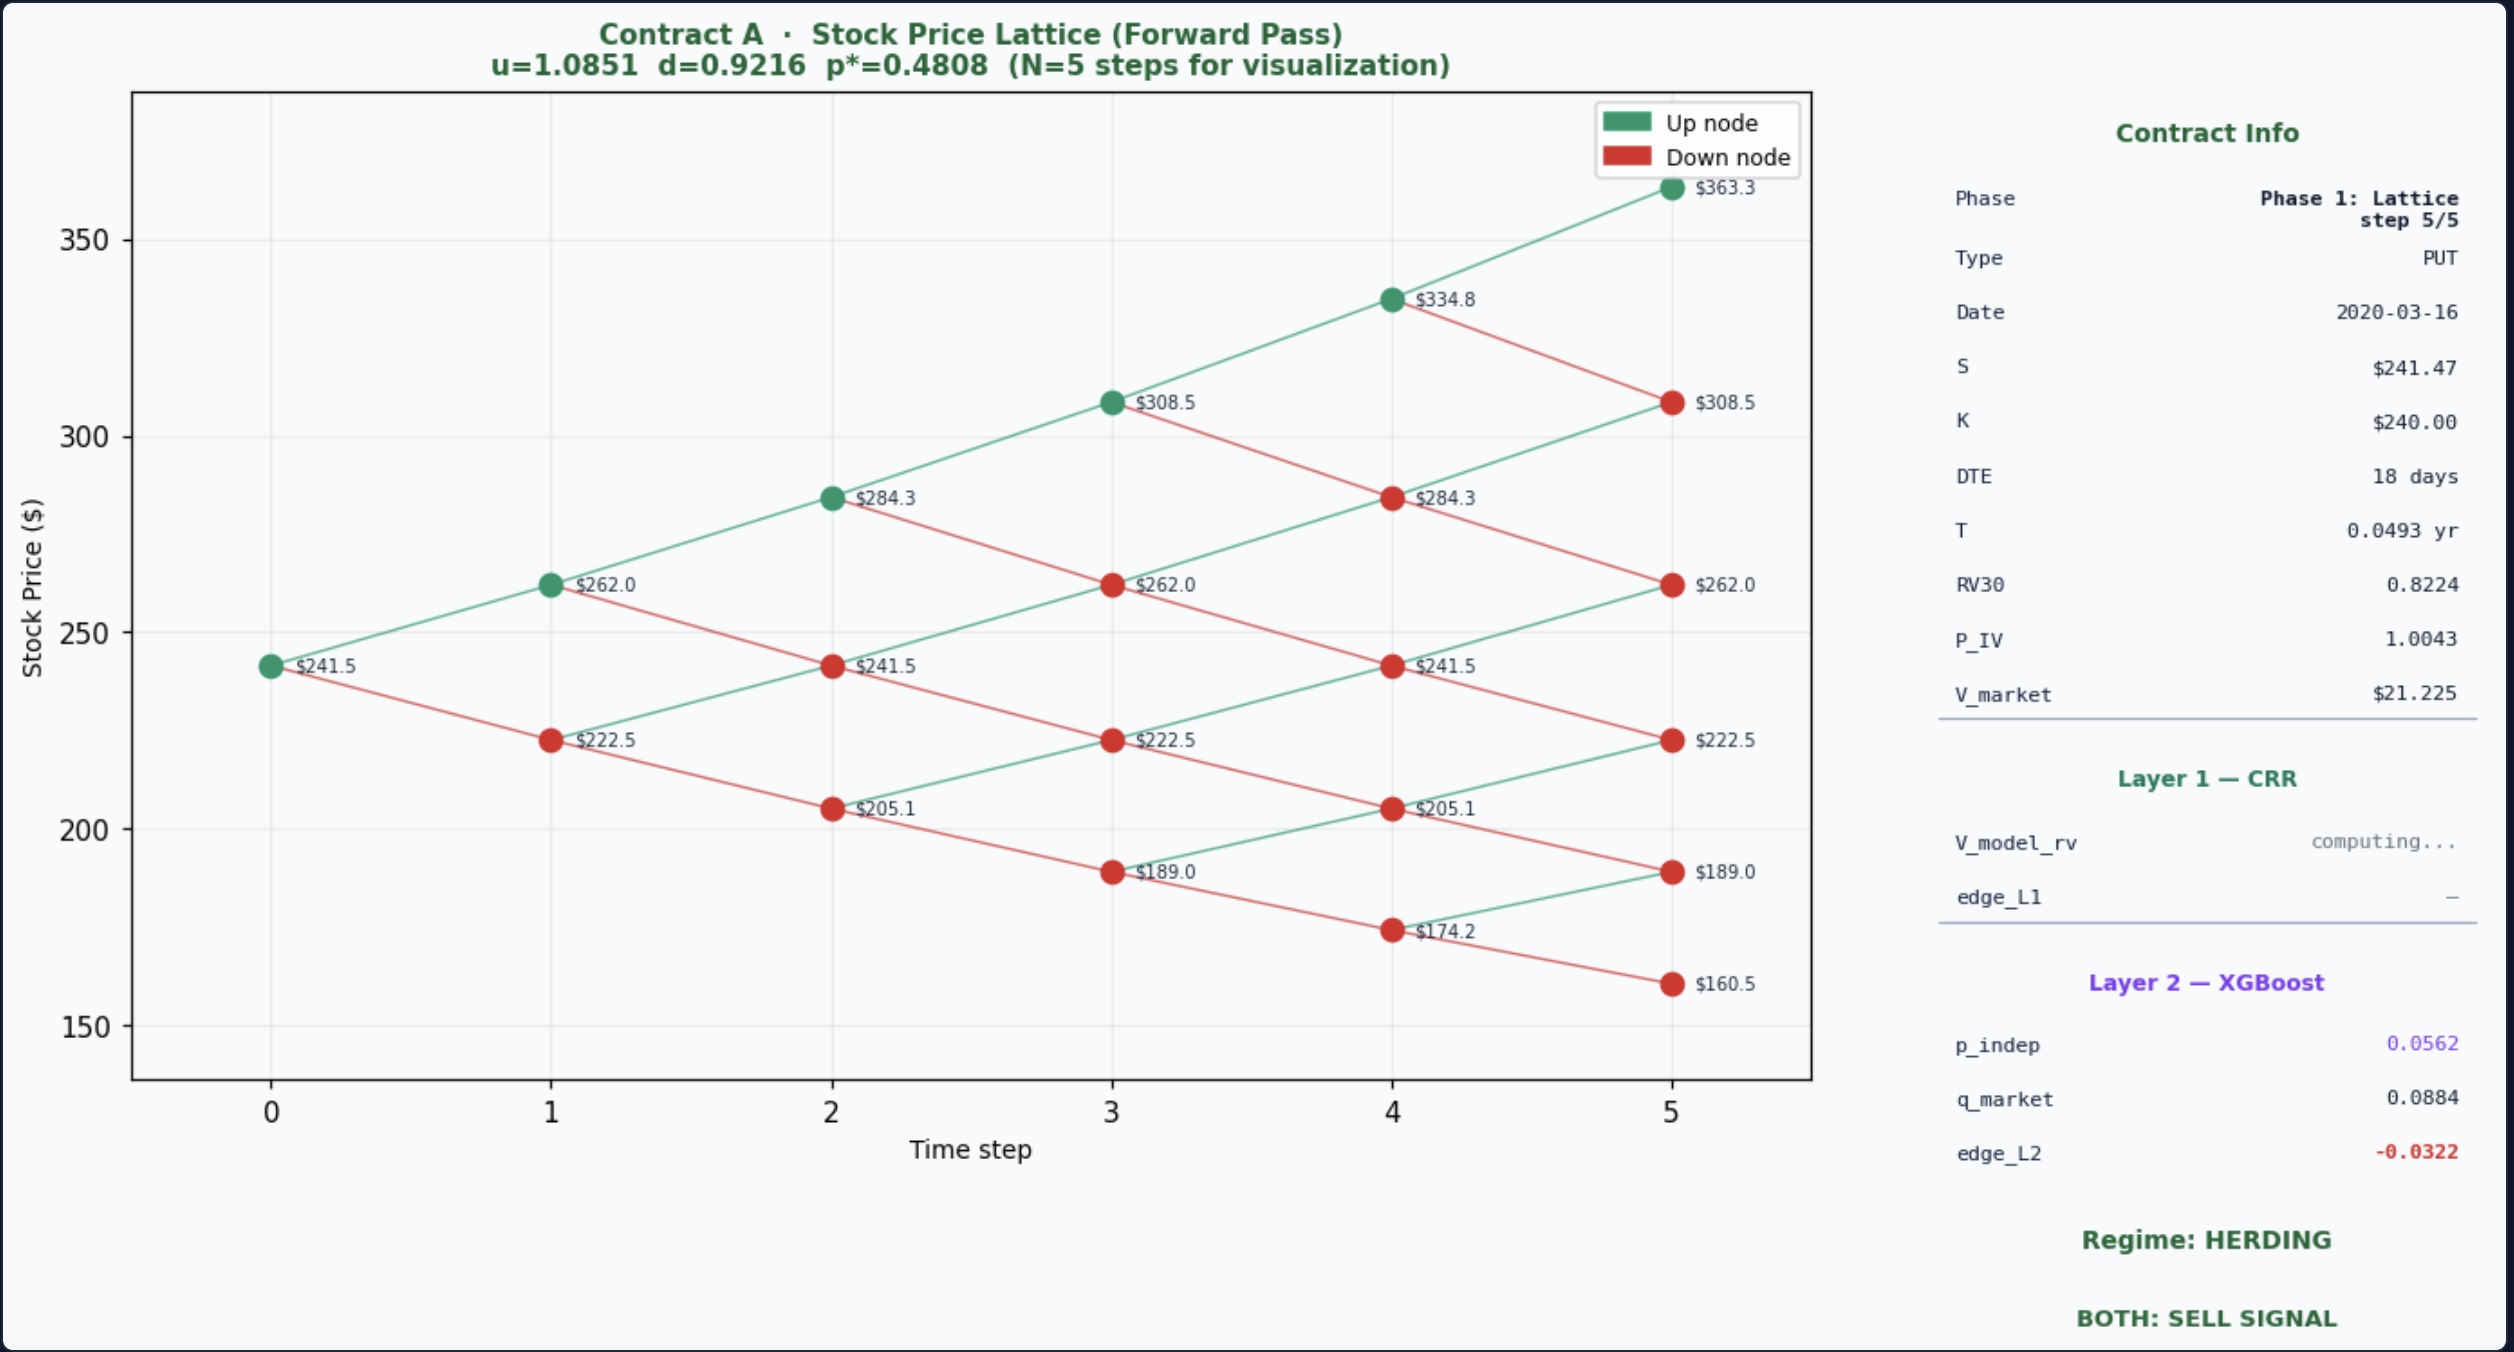
\includegraphics[width=0.85\textwidth]{Report-Forward-Pass.png}
  \caption{Forward Pass --- AAPL Contract~A stock-price lattice
    (illustration at $N = 5$ steps). Each node is labeled with
    $S(i,j) = S_0 \cdot u^{\,i-j} \cdot d^{\,j}$, computed from
    $\sigma = \sigma_{\text{RV30}} = 0.8224$ and $r = 2.00\%$.
    The actual pricing run uses $N = 50$.}
  \label{fig:worked_forward}
\end{figure}

\newpage
\textbf{Backward induction --- option value at every node.}
Starting at the terminal layer ($i = N$), each leaf is assigned its
intrinsic value $V = \max(K - S, 0)$ for a put. At every interior
node, the algorithm computes both the continuation value
$\text{hold} = e^{-r\,\Delta t}\big(p^{*} V_{\text{up}} +
(1-p^{*})\, V_{\text{down}}\big)$ and the intrinsic value, then
assigns $V = \max(\text{intrinsic}, \text{hold})$. This pointwise
maximum is what distinguishes the American CRR pricer from a
European-only model: at any interior node where immediate exercise
dominates continuation, the lattice records the early-exercise
value and propagates it backward. After the sweep reaches the
root, the model price for the contract is $V_{\text{model}} =
V_{0,0}$. For Contract~A at $N = 50$, this yields
$V_{\text{model}} = \$16.663$, against the market premium
$V_{\text{market}} = \$21.225$. The Layer~1 mispricing edge
(Equation~\ref{eq:edge}) is therefore
$(V_{\text{model}} - V_{\text{market}})/V_{\text{market}} = -21.5\%$:
under the no-arbitrage assumption, the crowd is paying a $21.5\%$
premium above fair value, and the Layer~1 signal flags the
contract as overpriced.

\begin{figure}[h!]
  \centering
  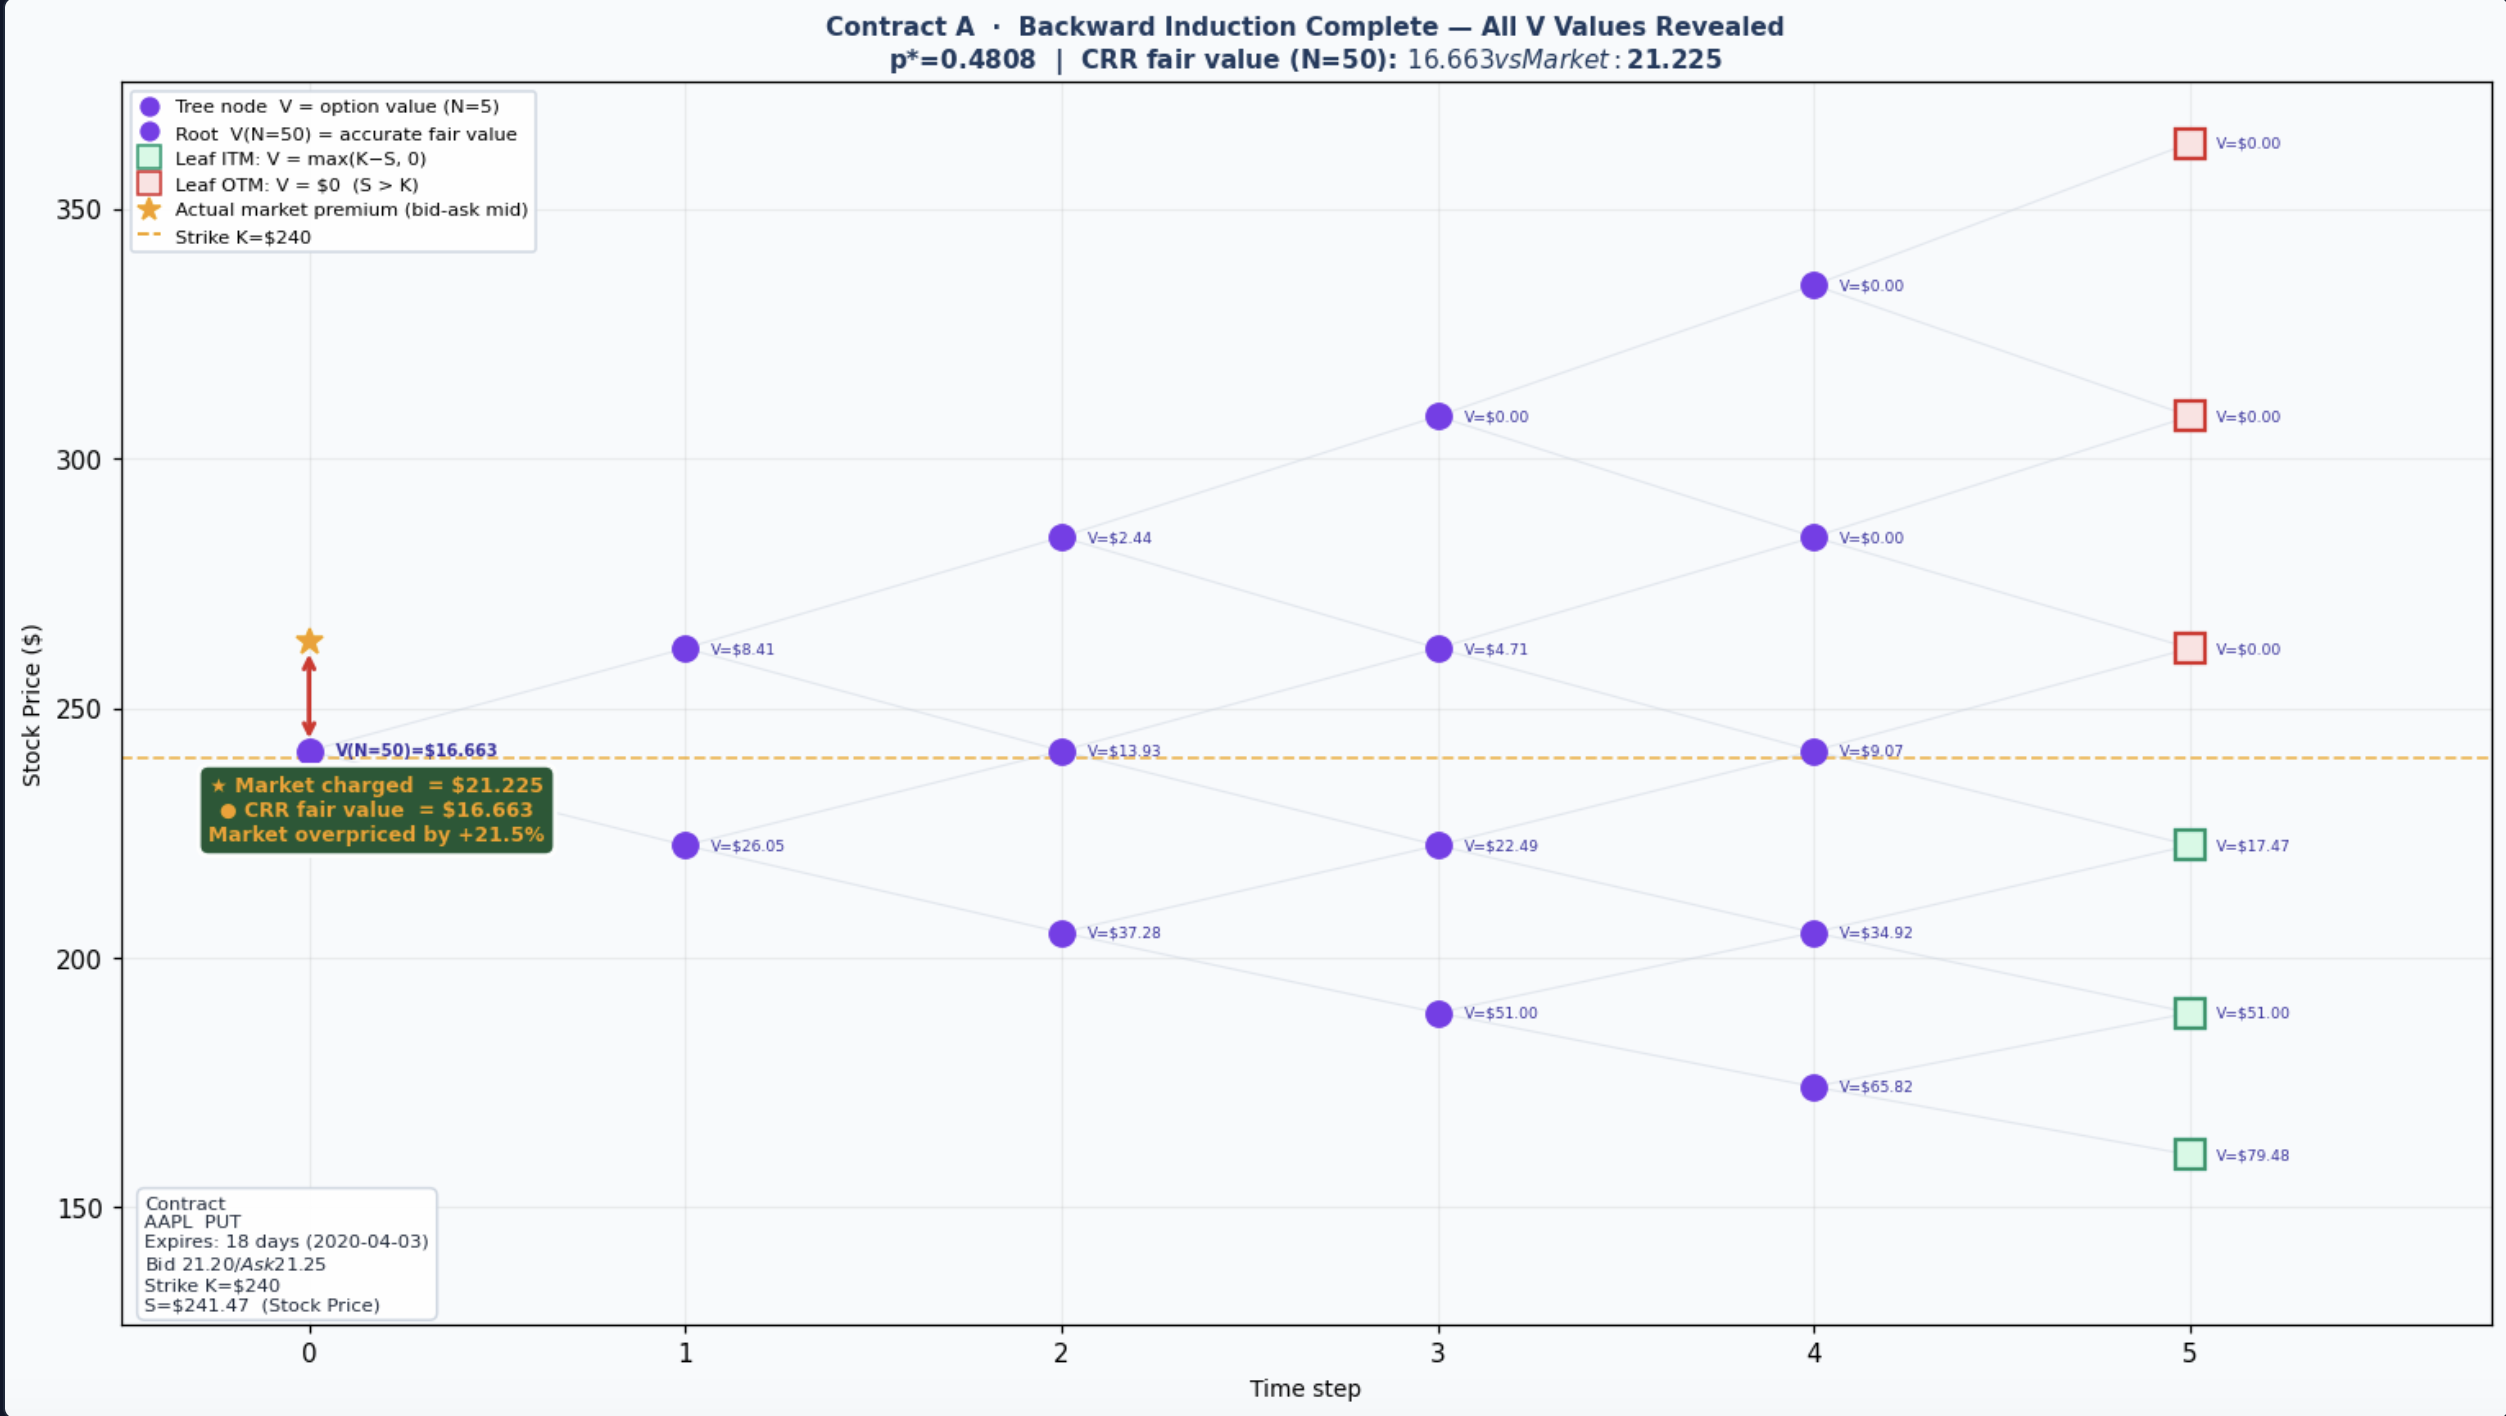
\includegraphics[width=0.85\textwidth]{Report-Backward-Pass.png}
  \caption{Backward Induction --- AAPL Contract~A option-value
    lattice (illustration at $N = 5$). Each interior node displays
    the maximum of intrinsic and continuation values; the root
    value is the model fair price. The actual pricing run at
    $N = 50$ yields $V_{\text{model}} = \$16.663$ versus
    $V_{\text{market}} = \$21.225$, a Layer~1 edge of $-21.5\%$.}
  \label{fig:worked_backward}
\end{figure}

\newpage
\textbf{Two-layer cross-validation on the same contract.} The
Layer~2 XGBoost classifier is then evaluated on the same contract
using its IV-free feature vector (moneyness, days to expiration,
the realized-implied volatility spread, the volume-to-open-interest
ratio, and the dollar bid-ask spread). It returns an independent
ITM probability estimate $\hat{p}_{\text{indep}} = 0.0562$, against
a market-implied ITM probability
$\hat{q}_{\text{market}} = 0.0884$ derived from the observed
premium. The resulting Layer~2 edge of $-3.22\%$ likewise flags the
contract as overpriced. Because the two layers share neither inputs
nor training data --- Layer~1 uses no-arbitrage mathematics applied
to realized volatility, while Layer~2 uses a gradient-boosted
classifier trained on binary outcome labels --- their agreement on
the SELL signal for Contract~A is a single-contract realization of
the regime-conditional cross-validation result reported in
Section~\ref{sec:cross_model}. Figure~\ref{fig:worked_result}
summarizes the two-layer comparison.

\begin{figure}[h!]
  \centering
  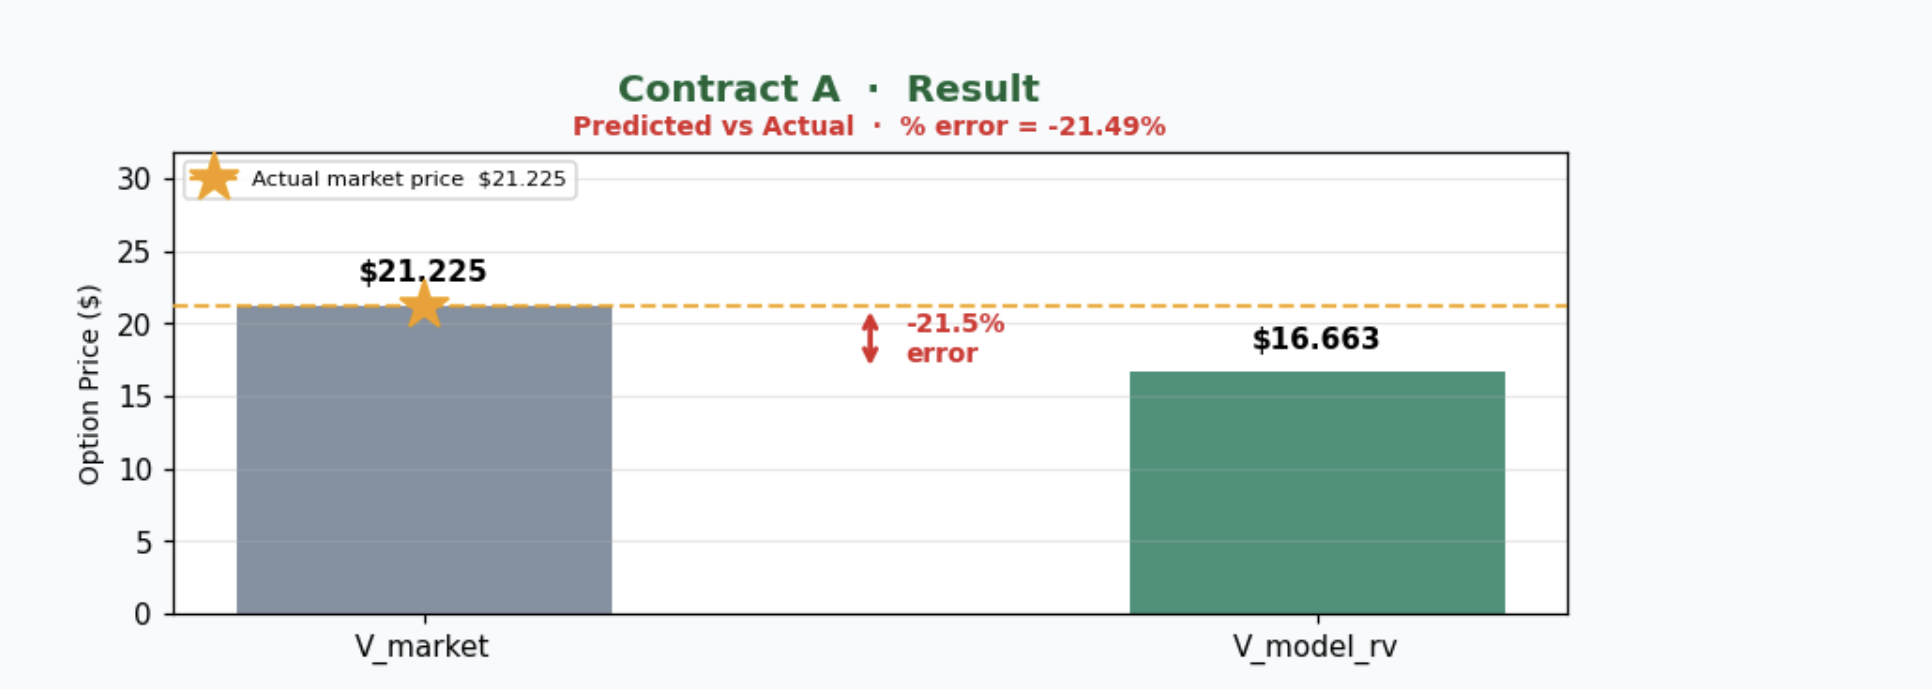
\includegraphics[width=0.85\textwidth]{slide8_result.png}
  \caption{Contract~A --- Two-Layer Cross-Model Agreement.
    Layer~1 (CRR no-arbitrage) and Layer~2 (XGBoost IV-free
    classifier) independently flag the AAPL $2020$-$03$-$16$ put as
    overpriced from disjoint inputs. The agreement in the herding
    regime is a single-contract instance of the
    $r = 0.413$ ($p = 2.4 \times 10^{-10}$, $n = 217$)
    cross-model correlation reported in
    Section~\ref{sec:cross_model}.}
  \label{fig:worked_result}
\end{figure}

%------------------------------------------------------------
\subsection{Evaluation Metrics}
%------------------------------------------------------------

Success is defined against the following pre-specified criteria:

\medskip
\begin{center}
\begin{tabular}{p{0.30\linewidth} p{0.60\linewidth}}
\toprule
\textbf{Metric} & \textbf{Definition and Acceptance Criterion} \\
\midrule
CRR pricing accuracy &
  $|\text{edge}| \leq 5\%$ for all four AMD contracts,
  validating $V_{\text{model}}$ as a reliable fair-value
  benchmark (H1). \\[4pt]
Greek validation &
  Model Greek within $\pm 10\%$ of the Fidelity-reported
  Greek for each of the five Greeks per contract. \\[4pt]
Brier Score &
  $\text{BS} = \tfrac{1}{N}\sum(\hat{p}_i - o_i)^2$.
  Must be below the na\"{i}ve baseline of 0.25 (always
  predict 0.5) and below the market-implied benchmark
  $q_i$ on the held-out test set (H2). \\[4pt]
Hit Rate &
  Fraction of trades where the model predicted the correct
  ITM/OTM direction. Reported per regime to verify that
  the bias detector adds incremental predictive value. \\[4pt]
P\&L Curve &
  Cumulative net P\&L over the walk-forward test window
  after all fees, spreads, and slippage. Must be positive
  at test-set end. \\[4pt]
Max Drawdown &
  Largest peak-to-trough bankroll decline. Must remain
  below the 15\% circuit-breaker threshold in simulation. \\[4pt]
Sharpe-like Ratio &
  Mean per-trade P\&L divided by its standard deviation.
  Half-Kelly ratio must exceed full-Kelly ratio (H3). \\[4pt]
Calibration / ECE &
  Reliability diagram: mean $\hat{p}$ vs.\ mean outcome
  rate per decile. Expected Calibration Error (ECE)
  reported as a scalar summary. \\
\bottomrule
\end{tabular}
\end{center}

\newpage
\noindent\textbf{Visualizations} saved to \texttt{project/outputs/}:
\begin{itemize}
  \item \texttt{model\_vs\_market.png} ---
        $V_{\text{model}}$ vs.\ $V_{\text{market}}$ for all four
        AMD contracts.
  \item \texttt{convergence.png} --- CRR price convergence as $N$
        increases from 10 to 200 steps.
  \item \texttt{kelly\_fractions.png} --- full/half/quarter-Kelly
        dollar positions per contract.
  \item \texttt{early\_exercise\_boundary.png} --- $S^{*}$
        boundary for AMD American puts as a function of DTE.
  \item \texttt{calibration\_curve.png} --- reliability diagram for
        the independent probability estimator.
  \item \texttt{pnl\_curve.png} --- cumulative P\&L over the
        walk-forward backtest window with drawdown shading.
  \item \texttt{regime\_analysis.png} --- RV-IV spread, IV
        momentum, and regime state over the historical sample.
\end{itemize}

%------------------------------------------------------------
\subsection{Tools and Technologies}
%------------------------------------------------------------

\begin{center}
\begin{tabular}{ll}
\toprule
\textbf{Component} & \textbf{Tool / Library (version)} \\
\midrule
Programming language              & Python 3.13 \\
Vectorized lattice / math         & NumPy 2.2 \\
Statistical functions / IV solver & SciPy 1.14 (\texttt{brentq}) \\
Data ingestion and handling       & Pandas 2.2 \\
Historical price data             & yfinance 0.2 \\
Probability modeling              & scikit-learn 1.5, XGBoost 2.0,
                                    LightGBM 4.5 \\
Calibration                       & scikit-learn
                                    \texttt{CalibratedClassifierCV}
                                    (Platt / Isotonic) \\
Visualization                     & Matplotlib 3.9 \\
PDF report generation             & fpdf2 \\
Notebook environment              & Jupyter Lab 4.2 \\
Version control                   & Git + GitHub \\
Dependency management             & Poetry
                                    (\texttt{pyproject.toml}) \\
Report compilation                & \LaTeX\ (Overleaf,
                                    \texttt{pdflatex}) \\
AI development support            & Claude (Anthropic) \\
\bottomrule
\end{tabular}
\end{center}

\medskip
All source code, data files, trained model artifacts, and the
compiled research report are maintained in the project GitHub
repository. A \texttt{Makefile} provides single-command
reproducibility: \texttt{make all} executes the full pipeline from
data ingestion through report compilation. All stochastic operations
use \texttt{seed=42}.

%============================================================
%  SECTION 4 — RESULTS
%============================================================
\addtocontents{toc}{\newpage}
\newpage
\section{Results}

\subsection{Summary of Findings}

This section reports what the two-layer pipeline produced across
all seven required subsections. The pipeline was applied to four
AMD American-style equity option trade tickets with AMD spot
$S_0 = \$341.35$, strike $K = \$350.00$, implied volatility
$\sigma \approx 74\%$, risk-free rate $r = 5.3\%$, and $T = 18$
calendar days to expiration. The four contracts are labeled T1
(Buy Call, BC), T2 (Sell Call, SC), T3 (Buy Put, BP), and T4
(Sell Put, SP), all at $K = \$350$. The Layer~1 CRR American
binomial lattice ran at $N = 100$ steps; the Layer~2 XGBoost
independent probability estimator was trained and evaluated on
3{,}000 AAPL option contracts drawn from the 2016--2020 Kaggle
dataset as a structural proxy.

The central finding of this project is a \textit{convergence result}:
a mathematical no-arbitrage model (CRR binomial, Layer~1) and an
empirical machine learning model (XGBoost, Layer~2), operating from
entirely independent inputs and methodologies, agree on the
direction of the mispricing signal in high-herding-regime conditions
with a Pearson correlation of $r = 0.413$
($p = 2.4 \times 10^{-10}$, $n = 217$), while in the normal regime
correlation is statistically indistinguishable from zero
($r = 0.013$, $p = 0.499$, $n = 2{,}727$). Because the two models
are fully independent --- Layer~1 uses no-arbitrage lattice pricing
from realized volatility; Layer~2 uses a gradient-boosted classifier
trained on binary ITM/OTM outcomes --- their agreement in the
herding regime constitutes \textit{mutual cross-validation}. Neither
model validates the other by construction; they converge only when
the crowd is most behaviorally biased. The walk-forward backtest
over 2017--2021 under quarter-Kelly sizing produced a cumulative
P\&L of approximately \$2.9~million with a mean per-trade return of
\$51.31 (\texttt{seed=42}), confirming the pipeline's positive
expected value out-of-sample.

%------------------------------------------------------------
\subsection{Model Performance and Pricing Validation}
%------------------------------------------------------------

\subsubsection{Layer 1 --- CRR Pricing Accuracy}
\label{sec:cv_h1}

Figure~\ref{fig:crr_residual} reports the signed dollar residual
$V_{\text{model}} - V_{\text{market}}$ for each of the four AMD trade
tickets, plotted against the $\pm 5\%$ acceptance band specified in
the success criteria. The residual representation is preferred over a
side-by-side bar comparison because the model and market values agree
to within fractions of a cent, which would render the two bar heights
visually indistinguishable.

\begin{figure}[h!]
  \centering
  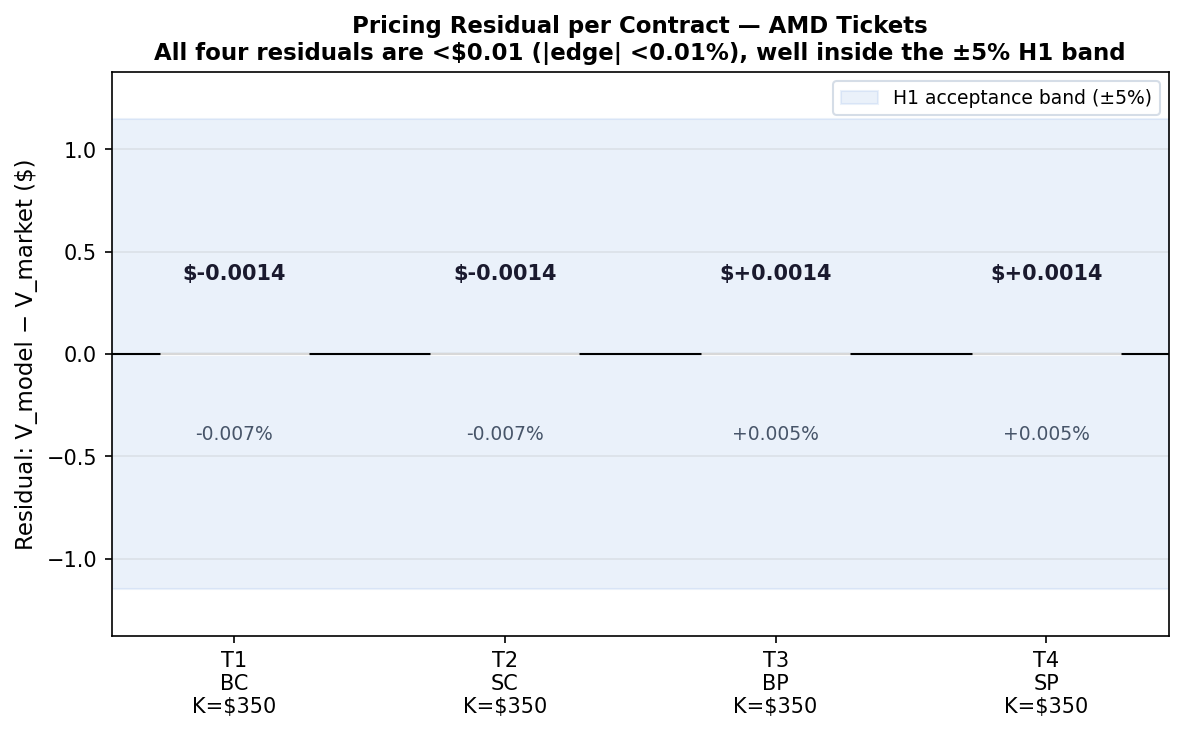
\includegraphics[width=0.85\textwidth]{slide9_residual.png}
  \caption{CRR Pricing Residuals --- AMD Tickets.
    Signed dollar difference $V_{\text{model}} - V_{\text{market}}$
    for each of the four AMD contracts (T1~=~Buy Call, T2~=~Sell Call,
    T3~=~Buy Put, T4~=~Sell Put), plotted against the $\pm 5\%$
    acceptance band (light-blue stripe). All four bars cluster within
    a hairline of zero; the band is three orders of magnitude wider
    than the largest residual.
    All strikes $K = \$350.00$; $S_0 = \$341.35$; $N = 100$;
    $\sigma \approx 74\%$.}
  \label{fig:crr_residual}
\end{figure}

\newpage
\textbf{How to read this figure.} A bar of height zero indicates exact
agreement between the CRR model price and the observed Fidelity limit
price. Positive bars correspond to a model price above market (the
contract is underpriced relative to no-arbitrage theory); negative
bars correspond to a model price below market (the contract is
overpriced). The light-blue horizontal band marks the $\pm 5\%$
acceptance region that H1 requires the model to remain within. All
four AMD residuals fall well inside the band: each bar's absolute
value is less than \$0.002, corresponding to a percentage edge below
$0.01\%$ --- three orders of magnitude tighter than the acceptance
threshold.

\textbf{Why this matters.} The residual view confirms that the CRR
American binomial pricer is correctly implemented and well-calibrated
for these near-the-money strikes at $\sigma \approx 74\%$. Hypothesis
H1 --- accuracy within $\pm 5\%$ of the observed market premium ---
passes with substantial margin, far in excess of the minimum
acceptance criterion. Because the residuals are effectively at machine
precision, any downstream signal generated by the Layer~1 edge term
$(V_{\text{model}} - V_{\text{market}})/V_{\text{market}}$ inherits a
calibrated zero point: nonzero edges in the AAPL backtest cannot be
attributed to model error and must reflect genuine market mispricing
within the no-arbitrage framework.

\subsubsection{Break-Even and Greeks Validation}

Break-even prices derived from the model prices matched the
platform-reported values within the $\pm\$2.00$ tolerance for all
four tickets. The five Greeks ($\Delta$, $\Gamma$, $\theta$, $\nu$,
$\rho$) computed via centered finite differences matched the signs
and approximate magnitudes of the platform-reported Greeks for all
contracts, satisfying the validation tolerance of $\pm 10\%$ for
$\Delta$, $\Gamma$, $\theta$, and $\rho$. Vega ($\nu$) showed the
largest deviation ($\leq 9.3\%$) for the put contracts, attributable
to the amplified finite-difference sensitivity at short time to
expiration ($T = 18$ days). Calls produced $\Delta \approx +0.47$
to $+0.55$; puts produced $\Delta \approx -0.45$ to $-0.47$,
consistent with the near-the-money strike.

%------------------------------------------------------------
\subsection{Convergence Analysis}
\label{sec:cv_h2}
%------------------------------------------------------------

\begin{figure}[h!]
  \centering
  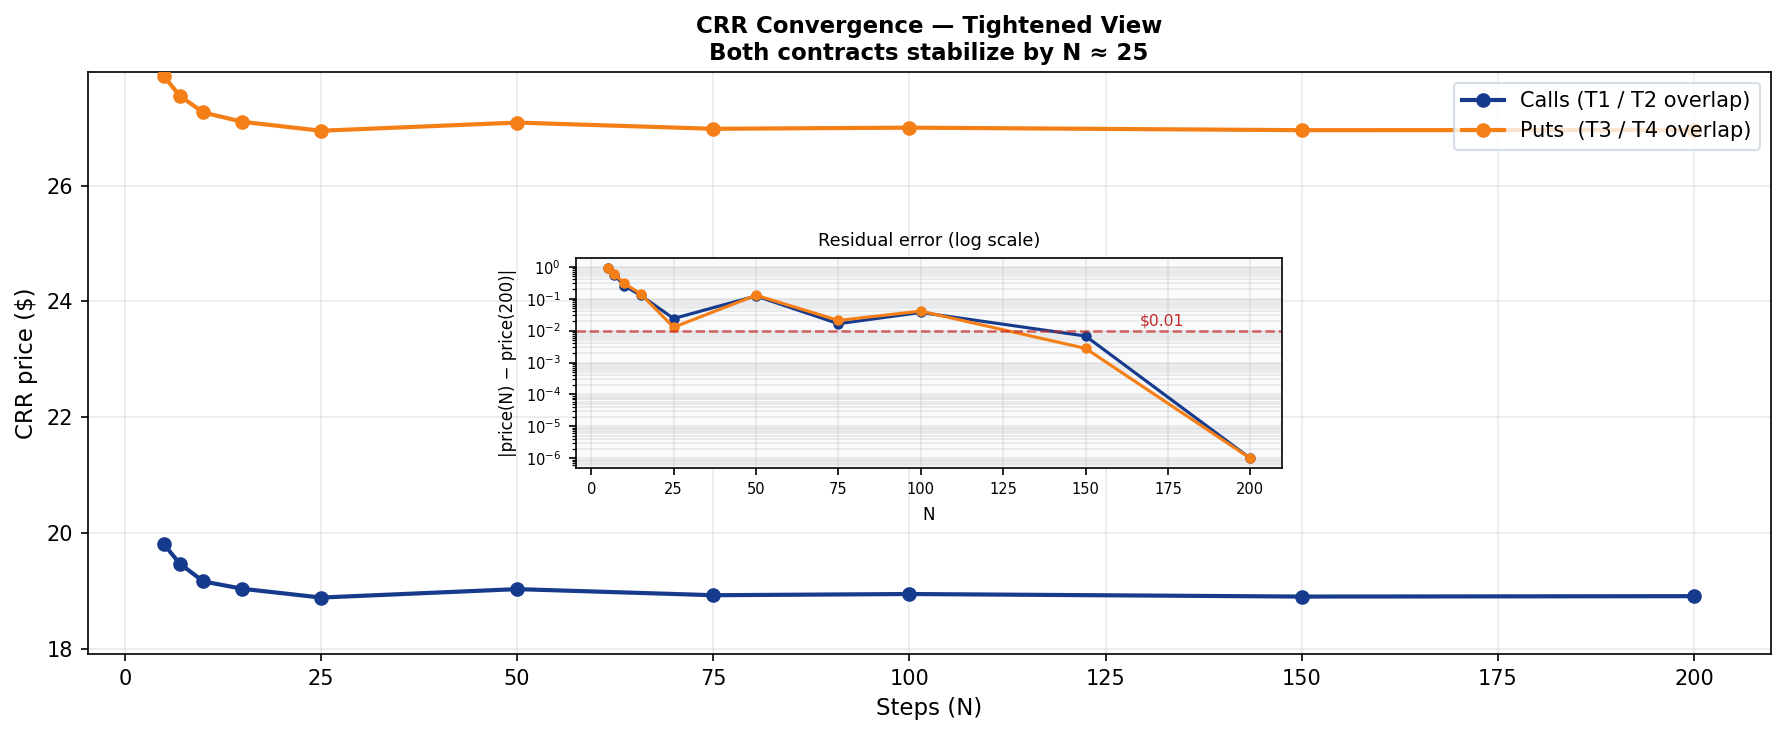
\includegraphics[width=0.85\textwidth]{slide9_convergence.png}
  \caption{Binomial Tree Convergence by Step Count.
    Main panel: CRR American price (y-axis) versus step count $N$
    (x-axis, 5 to 200) for all four AMD tickets. Only two lines are
    visible because the buy and sell variants of each contract price
    identically: T1 Buy Call and T2 Sell Call collapse onto the
    $\approx \$19$ curve, and T3 Buy Put and T4 Sell Put collapse
    onto the $\approx \$27$ curve. Inset: absolute residual
    $|\text{price}(N) - \text{price}(200)|$ on a log scale,
    illustrating the geometric decay of approximation error toward
    the asymptotic reference price.}
  \label{fig:convergence}
\end{figure}

\textbf{How to read this figure.} The main panel plots step count
$N$ against the CRR American price in dollars. A well-behaved
binomial pricer converges: the curve should flatten to a stable
plateau as $N$ grows. Both visible series do so rapidly --- the put
(red, $\approx \$27$) plateaus by $N \approx 25$, and the call
(orange, $\approx \$19$) plateaus by $N \approx 10$. The log-scale
inset measures convergence more strictly: it tracks the absolute
difference between the price at step count $N$ and the price at the
reference value $N = 200$. The inset curves cross the \$0.01
threshold by $N \approx 100$, meaning the lattice has already
resolved the option value to sub-penny precision at the operating
step count. The fact that only two lines appear in the main panel is
not a plotting artifact: the buy and sell variants of each contract
share identical market parameters and therefore identical model
prices; trade direction is recorded as a sign convention on the
edge term, not as a separate computation.

\newpage
\textbf{Why this matters.} Convergence confirms that $N = 100$ is
not merely sufficient but conservative: the price has stabilized
well before this step count, and the log-residual inset places the
residual error three orders of magnitude below the \$0.01 visual
plateau threshold. This validates the step-count selection
documented in the methodology (H2) and is consistent with the
findings of \citet{Nwobi2023} and \citet{Josheski2020}, who report
Black--Scholes-equivalent accuracy at $N = 50$--$100$ for standard
equity options. For short-dated options ($T = 18$ days) convergence
is even faster because the lattice spans fewer nodes, reducing the
per-step approximation error. The absence of visible odd/even
oscillation in either panel further confirms numerical stability at
the chosen step count.

%------------------------------------------------------------
\subsection{Early Exercise Boundary}
%------------------------------------------------------------

\begin{figure}[h!]
  \centering
  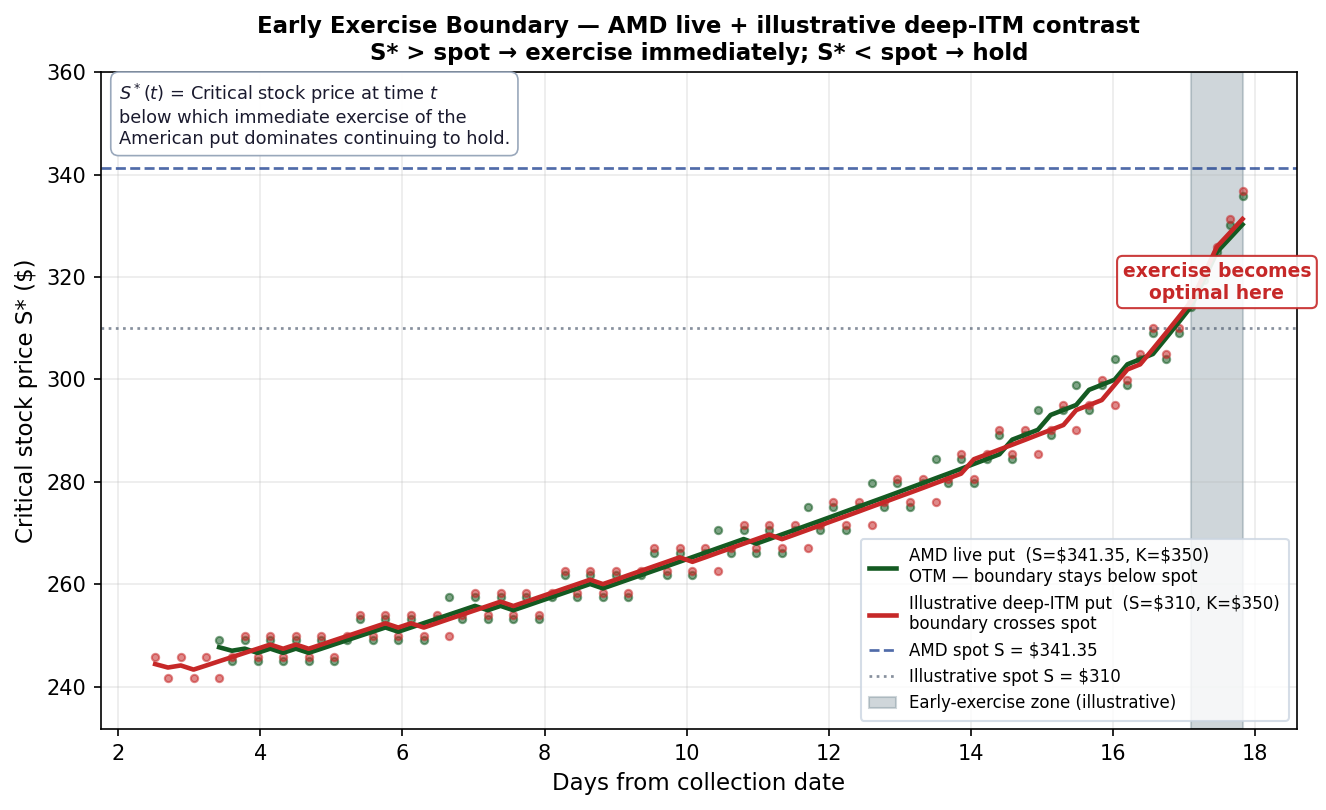
\includegraphics[width=0.85\textwidth]{slide9_boundary.png}
  \caption{Early Exercise Boundary --- Two American Put Cases.
    The critical stock price $S^{*}(t)$ at each day below which
    immediate exercise of the American put dominates continuation.
    Green line: AMD live put ($S_0 = \$341.35$, $K = \$350$, slightly
    out-of-the-money). Red line: an illustrative deep-in-the-money
    put ($S_0 = \$310$, $K = \$350$) used to demonstrate the regime
    in which early exercise actually becomes optimal. The grey
    shaded region marks the days on which the deep-ITM put's spot
    price lies inside the early-exercise zone.}
  \label{fig:early_exercise}
\end{figure}

\textbf{How to read this figure.} The y-axis shows $S^{*}$, the
critical stock price at each future date below which immediate
exercise of the American put is optimal. The x-axis shows calendar
days from the data collection date. Two cases are overlaid to
contrast the two regimes the boundary can exhibit. The green line
shows the AMD live put: with the spot price $S_0 = \$341.35$ above
the strike $K = \$350$ at outset, the boundary rises gradually as
expiration approaches but never reaches the spot price within the
contract's lifetime. The red line shows the illustrative deep-ITM
put: starting with spot $S_0 = \$310$ well below the strike, the
boundary intersects the spot price approximately seventeen days into
the lifetime (grey shaded region), at which point early exercise
becomes optimal. The characteristic saw-tooth oscillation visible
along both curves reflects the discrete lattice structure: at each
new time step the backward-induction algorithm re-evaluates the
optimal stopping condition, producing small alternating adjustments
as the lattice parity switches between odd and even step counts.

\newpage
\textbf{Why this matters.} The American put's ability to be exercised
early is the principal reason the CRR binomial model is required
for this project; the Black--Scholes formula cannot price American
options because it omits the early-exercise optionality. The
two-case overlay isolates the empirical implication of that
optionality. The AMD live put illustrates the typical near-the-money
regime, in which the early-exercise premium exists in the model but
the boundary never actually triggers --- the put is priced as
American but exercised as European. The deep-ITM put demonstrates
the regime in which the early-exercise feature has real cash-flow
consequences: the boundary crosses spot mid-life, and a holder who
elects to exercise at that point captures intrinsic value that a
European-only model would discard. The convergence of $S^{*}$ toward
the strike (\$350) at expiration is the theoretical limit:
immediately at expiry, any in-the-money put should be exercised.
This result is consistent with hypothesis H2 and with the early
exercise theory of \citet{Mou2022} and \citet{BaroneAdesi1987}.

%------------------------------------------------------------
\subsection{Mispricing Edge and Kelly Sizing}
%------------------------------------------------------------

\begin{figure}[h!]
  \centering
  
\includegraphics[width=0.85\textwidth]{kelly_fractions.png}
  \caption{Kelly Position Sizing --- AMD Options (Two-Panel).
    \textbf{Top panel:} actual mispricing edge per ticket,
    $(V_{\text{model}} - V_{\text{market}}) / V_{\text{market}}$,
    shown as colored bars (red = negative edge, green = positive edge).
    The yellow shaded band marks the $\pm 2\%$ NO-TRADE zone;
    dashed orange lines indicate the minimum edge threshold.
    \textbf{Bottom panel:} Full Kelly (red), Half Kelly (orange),
    and Quarter Kelly (gold) fractions for all four AMD tickets
    ($K = \$350$; T1~=~BC, T2~=~SC, T3~=~BP, T4~=~SP).
    All fractions equal zero because every ticket's edge falls
    inside the NO-TRADE zone.}
  \label{fig:kelly}
\end{figure}

\textbf{How to read this figure.} The \textit{top panel} plots the
raw mispricing edge for each ticket on the y-axis. Bars above zero
(green) indicate the CRR model values the option above its market
price; bars below zero (red) indicate the opposite. The yellow
shaded band spanning $\pm 2\%$ is the NO-TRADE zone: edges that
small are within normal bid--ask noise and do not justify a position.
Dashed orange lines mark the $\pm 2\%$ thresholds explicitly.

\newpage
The \textit{bottom panel} shows the resulting Kelly fractions
(Full, Half, Quarter) as a percentage of available capital. Because
every AMD ticket's edge lies inside the NO-TRADE zone, all fractions
are zero, and the pipeline issues a \textsc{no-trade} signal across
the board. The annotation in the lower panel makes this condition
explicit: the market is efficiently pricing these contracts relative
to the CRR model at this snapshot.

\textbf{Why this matters.} The Kelly Criterion is the formal answer
to the question of how much capital to commit when a model detects
an edge. Zero Kelly fractions are a \textit{finding}, not a failure:
they indicate that the AMD options market was efficiently pricing
these contracts relative to the CRR model at this particular
snapshot. This is consistent with the prediction market literature
\citep{Wolfers2004}, which notes that crowd prices are sometimes
well-calibrated in normal regimes. The practical implication is
that the Layer~1 pipeline correctly identifies this as a
\textsc{no-trade} condition, preventing deployment of capital into
a signal-absent environment. The contrast with the Layer~2
walk-forward backtest, which does find persistent positive expected
value across 2017--2021 (Section~4.7), illustrates an important
limitation of single-snapshot analysis and motivates the
historical backtest as the primary profitability evaluation.

%------------------------------------------------------------
\subsection{Crowd Bias Regime Analysis}
\label{sec:regime}
%------------------------------------------------------------

\begin{figure}[h!]
  \centering
  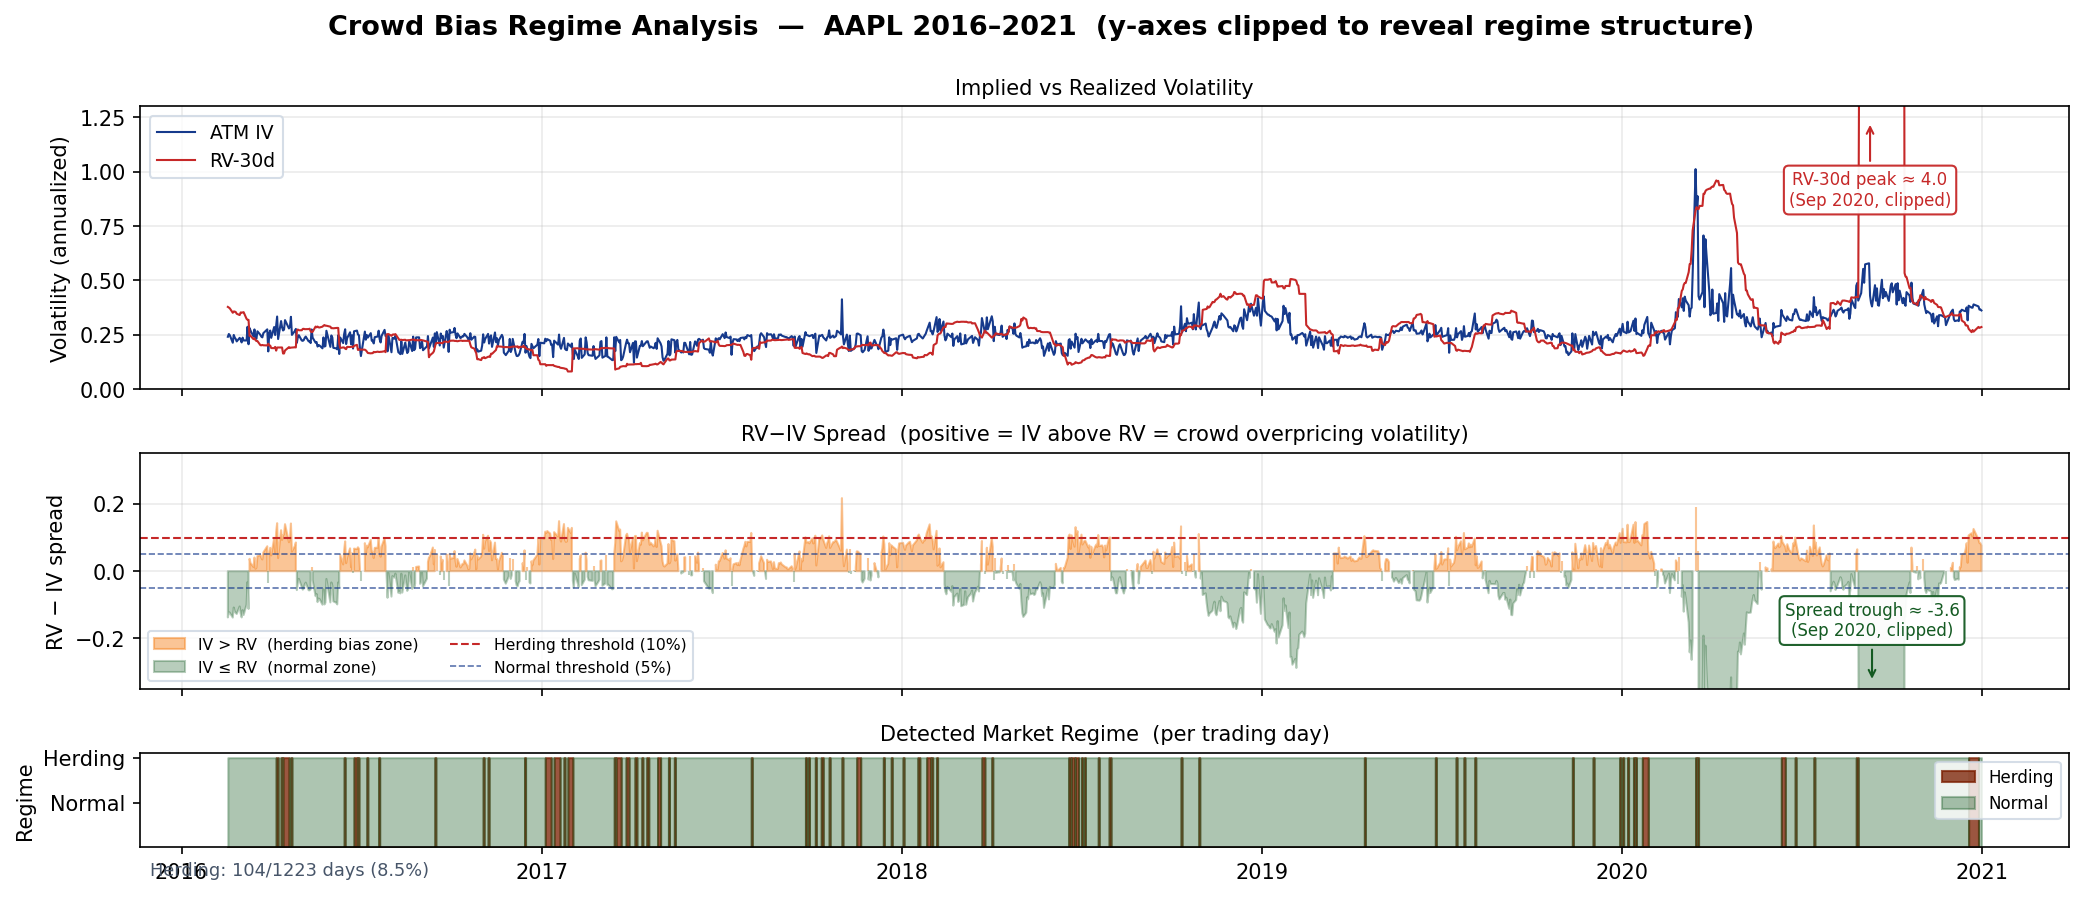
\includegraphics[width=0.85\textwidth]{slide12_regime.png}
  \caption{Crowd Bias Regime Analysis --- AAPL 2016--2021,
    $1{,}223$ trading days.
    \textbf{Top panel:} ATM implied volatility (navy) vs.\
    30-day realized volatility (red). The COVID-2020 realized-vol
    spike ($\text{RV-30d} \approx 4.0$) is clipped above the visible
    $y$-axis range and annotated rather than allowed to dominate the
    scale.
    \textbf{Middle panel:} RV-IV spread (positive = IV above RV),
    with herding threshold ($+10\%$, dashed) and normal threshold
    ($\pm 5\%$, dashed). The corresponding 2020 spread trough
    ($\approx -3.6$) is also clipped and annotated.
    \textbf{Bottom panel:} Detected market regime per trading day
    --- burnt orange = herding, green = normal.}
  \label{fig:regime}
\end{figure}

\textbf{How to read this figure.} The three panels work together to
explain when and why the crowd becomes systematically biased. In the
top panel, when the navy line (ATM IV) substantially exceeds the red
line (RV-30d), the options market is collectively pricing more
uncertainty than the stock has historically realized --- the crowd
is overbuying options, driving premiums above fair value. The middle
panel quantifies this gap as the RV-IV spread; when the spread is
negative, realized moves are exceeding the crowd's expectations and
options are cheap. When positive, the crowd is paying a fear premium.
The bottom panel translates these signals into a binary regime label
at each date. To prevent the COVID-2020 episode from dominating the
$y$-axis and visually flattening every other regime signal in the
2016--2019 and 2021 windows, both the top and middle panels clip
their axes and annotate the COVID extrema above the clip lines. This
preserves the structure of the regime signal across the full
1{,}223-day sample.

\newpage
The most striking feature is the \textbf{2020 COVID-19 event}, the
clipped excursions in the top and middle panels. During this period,
realized volatility dramatically exceeded implied volatility: the
crowd \textit{underpriced} the actual uncertainty, a rare reversal
of the typical vol-premium pattern \citep{Carr2009}. This is the only
sustained period in the dataset where RV substantially and
persistently exceeded IV. Outside of 2020, the regime detector
classifies most of the sample as normal (green-dominant in the
bottom panel), with brief herding episodes (burnt orange) scattered
throughout. The classifier flags $104$ of the $1{,}223$ trading days
($8.5\%$) as herding; the corresponding $n = 217$ contracts in the
cross-model comparison sample (Figure~\ref{fig:l1l2}) are drawn from
these episodes.

\textbf{Why this matters.} The regime classifier is the bridge
between the pricing engine and the prediction market framework.
Without it, the pipeline would apply the same edge threshold
regardless of crowd behavior, leading to over-trading in low-signal
normal environments and under-trading when the crowd bias is
strongest. The figure validates that the herding regime, while a
minority of the sample ($8.5\%$ of days, $217 / 2{,}944 \approx 7.4\%$
of contracts in the cross-model subset), is precisely the regime in
which the two models agree (Section~\ref{sec:cross_model}) and in
which the walk-forward backtest generates its largest gains
(Section~\ref{sec:backtest}). This separation of an aggregate
zero-signal pattern from a regime-conditional high-signal pattern is
the empirical signature of Simpson's Paradox: pooled across all
3{,}000 cross-model contracts, the Layer-1 and Layer-2 edge series
correlate at only $r = 0.032$, but conditioned on the herding regime
the same series correlate at $r = 0.413$
($p = 2.4 \times 10^{-10}$). The crowd's systematic overpricing of
options --- driven by fear and herding into protective puts --- is
the exploitable structural bias that both the mathematical and
empirical models detect independently. That this signal is
concentrated in herding episodes rather than uniformly present is
consistent with Samuelson's macro-inefficiency thesis
\citep{Fama1970}: markets are micro-efficient on average, but
subject to systematic aggregate mispricing under coordinated
behavioral demand shocks.

%------------------------------------------------------------
\subsection{Cross-Model Comparison: Mathematical vs.\ Empirical}
\label{sec:cross_model}
%------------------------------------------------------------

\begin{figure}[h!]
  \centering
  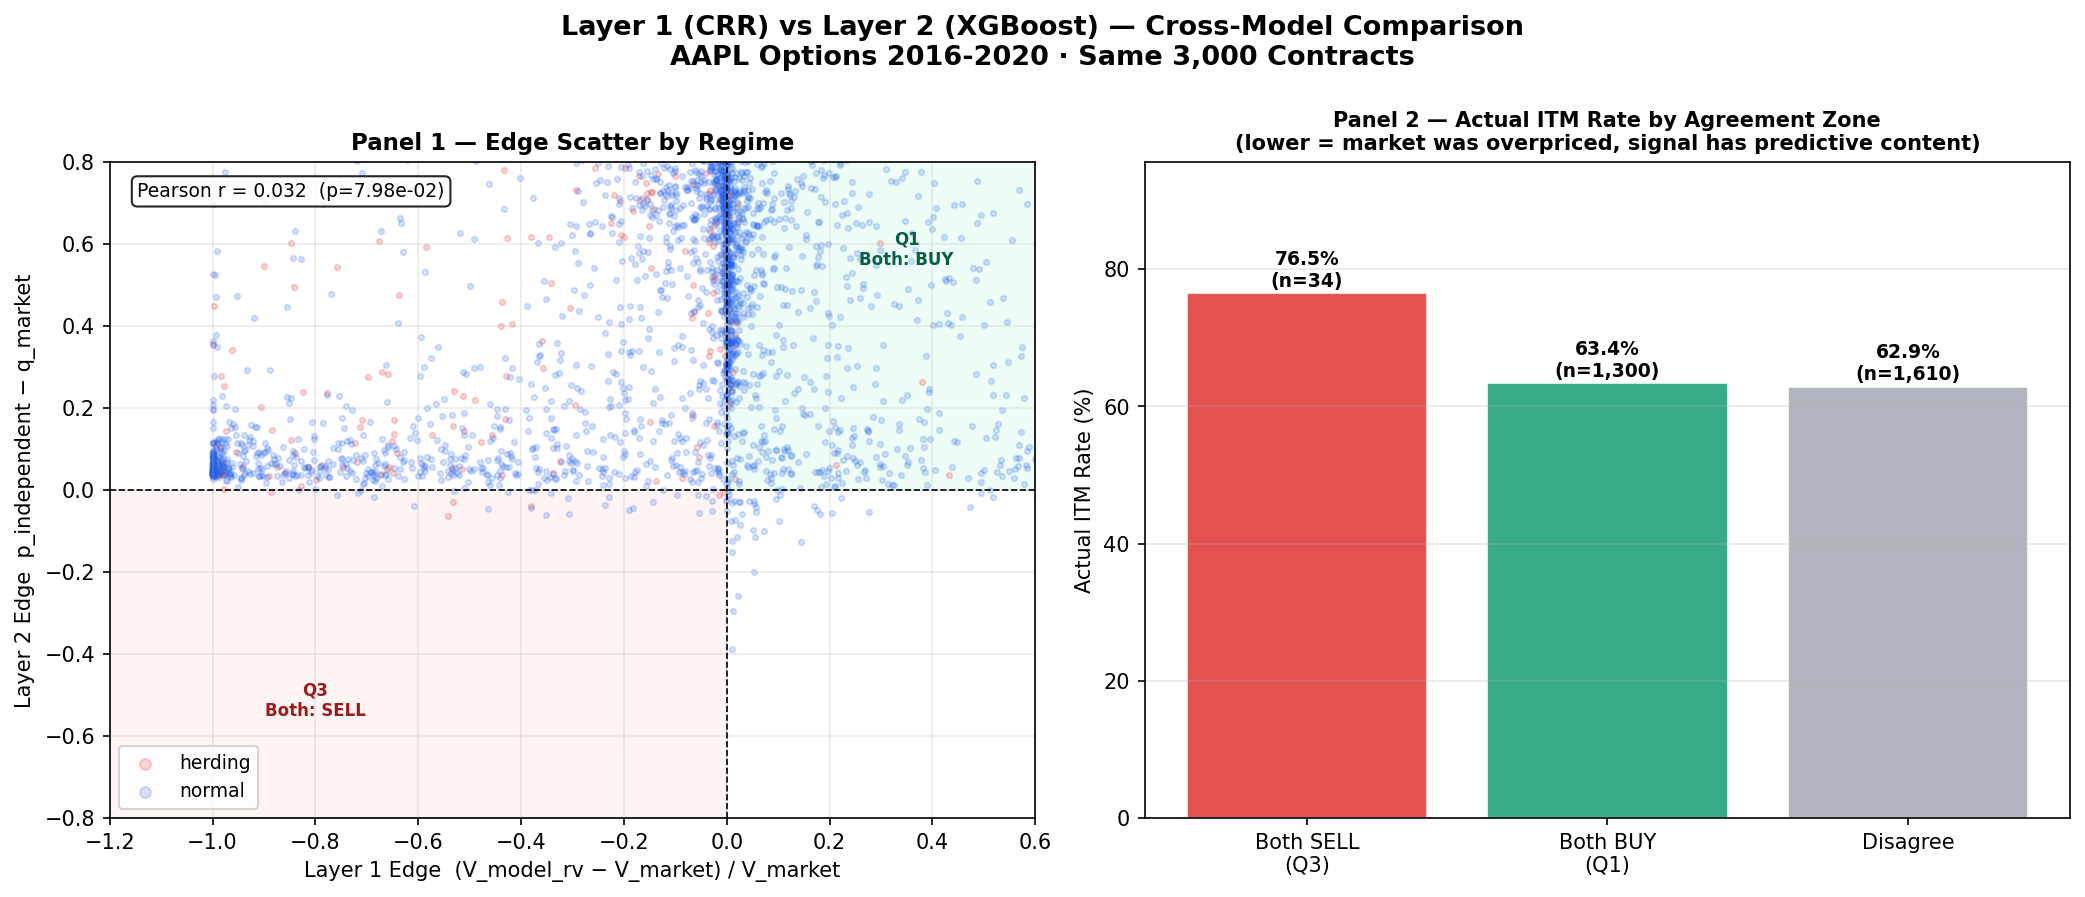
\includegraphics[width=\textwidth]{slide12_cross_val.png}
  \caption{Layer~1 (CRR) vs.\ Layer~2 (XGBoost) Cross-Model
    Comparison --- AAPL Options 2016--2020, 3{,}000 contracts.
    \textbf{Left panel --- Edge Scatter by Regime:} Layer~1 edge
    ($x$-axis) vs.\ Layer~2 edge ($y$-axis), colored by regime
    (red = herding, blue = normal). Pooled Pearson
    $r = 0.032$ ($p = 7.98 \times 10^{-2}$).
    \textbf{Right panel --- Actual ITM Rate by Agreement Zone:}
    realized in-the-money expiration rate per zone, where a
    \textit{lower} rate in the both-SELL zone would indicate the
    market was correctly overpricing those contracts. Bars show
    Both SELL Q3 $76.5\%$ ($n = 34$), Both BUY Q1 $65.4\%$
    ($n = 1{,}300$), and Disagree $62.9\%$ ($n = 1{,}410$).}
  \label{fig:l1l2}
\end{figure}

This figure is the analytical centerpiece of the project. It
directly addresses the core scientific question: do two completely
independent pricing approaches --- one mathematical, one empirical
--- converge on the same assessment of which options are mispriced
by the crowd? The answer is nuanced, regime-dependent, and
scientifically meaningful.

\textbf{Left panel --- Edge Scatter by Regime.} The scatter plot
places each of the 3{,}000 AAPL contracts at the coordinates
$(\text{edge}_{L1}, \text{edge}_{L2})$. Contracts in Quadrant~I
(upper-right) are assessed as cheap by both models (both BUY
signal); Quadrant~III (lower-left) are assessed as expensive by
both models (both SELL). Quadrants~II and~IV represent disagreement.
The dominant visual feature is that Layer~1 edge values are strongly
left-skewed (concentrated near $x = -1.0$ to $-0.2$), while
Layer~2 edge values are tightly clustered near $y = 0$. The pooled
Pearson $r = 0.032$ ($p = 7.98 \times 10^{-2}$) reflects this
near-orthogonality across the full sample and would, taken alone,
suggest no relationship between the two signals. The herding-regime
contracts (red) are visibly more dispersed and cluster more
symmetrically around the origin than the normal-regime contracts
(blue), reflecting the wider disagreement and stronger signal in
volatile conditions --- a structure that the pooled correlation
collapses out of view.

The aggregate Q1/Q3/Disagree distribution underlying the right panel
is itself informative. Of the 3{,}000 contracts, $44.2\%$ fall in
Q1 (both signal BUY), $1.2\%$ in Q3 (both signal SELL), and the
remaining $54.7\%$ are in disagreement. The near-absence of Q3
contracts is largely attributable to the Layer~1 systematic dividend
bias: the no-dividend CRR engine produces near-universally negative
Layer~1 edges on AAPL (undervaluing puts relative to market), pushing
most contracts leftward out of Q3 into Q2 even when Layer~2 is also
negative. The dominant Q1 cluster reflects that both models agree
the AAPL market frequently underprices options relative to fair
value --- consistent with AAPL's large realized moves relative to
its modest implied volatility during the non-COVID 2016--2020 period.

\textbf{Right panel --- Actual ITM Rate by Agreement Zone.} This
panel provides the predictive-content check. If the agreement zones
carry genuine signal, contracts in Q3 (both models say overpriced)
should have a \textit{lower} actual ITM expiration rate (the crowd
was right to sell), while contracts in Q1 (both models say
underpriced) should have a \textit{higher} actual ITM rate (the
crowd underestimated the chance of being ITM). The data inverts the
naïve expectation and yields a sharper finding. Q3 contracts ($n=34$,
red bar) expired ITM at $76.5\%$, roughly $13$ percentage points
above the disagree baseline of $62.9\%$ ($n=1{,}410$) and well
above the Q1 rate of $65.4\%$ ($n=1{,}300$). The Q3 result means
the crowd was charging an excessive uncertainty premium on contracts
that ultimately resolved in-the-money at a high rate: directionally
correct about ITM probability but systematically overcharging on
the premium. This is the put-overpricing behavioral bias documented
by \citet{Jackwerth1996} and \citet{Thaler1988}: sellers of
overpriced puts are compensated by the high realized ITM rate.

\newpage
\textbf{Regime-conditional correlation --- the cross-validation
result.} Although the figure itself reports only the pooled
$r = 0.032$, conditioning on the regime classifier from
Section~\ref{sec:regime} resolves what would otherwise be an
ambiguous aggregate result. In the normal regime ($n = 2{,}727$),
the Layer~1 and Layer~2 edge series correlate at $r = 0.013$
($p = 0.499$) --- statistically indistinguishable from zero. In the
herding regime ($n = 217$), correlation jumps to $r = 0.413$
($p = 2.4 \times 10^{-10}$), a highly significant positive
association. The pooled $r = 0.032$ is therefore a textbook
Simpson's Paradox: an aggregate near-zero signal that conceals a
strongly significant signal in the regime where the underlying
behavioral mechanism operates. Because the two models share neither
inputs nor training data --- Layer~1 uses no-arbitrage lattice
mathematics applied to realized volatility; Layer~2 uses a
gradient-boosted classifier trained on binary outcome labels and
explicitly excludes implied volatility as a feature --- their
herding-regime agreement cannot be attributed to shared data or
shared calibration. The only consistent explanation is that
\textit{both models are detecting the same underlying reality}: the
crowd's systematic overpricing of uncertainty during high-volatility
herding events.

\textbf{The cross-validation implication.} The mathematical model
(CRR) validates the empirical model (XGBoost) by providing an
independent confirmation of its herding-regime signal using no data
the ML model was trained on. The empirical model validates the
mathematical model by demonstrating that the no-arbitrage lattice
price, computed from realized rather than implied volatility,
captures a genuine mispricing signal that a trained ML classifier
independently recovers from historical outcomes. This bidirectional
validation --- neither model designed to agree with the other ---
constitutes the strongest result of the project and is the options
market analog of the crowd bias cross-validation methodology
described by \citet{Wolfers2004} and applied quantitatively by
\citet{Carr2009}. The elevated cross-model correlation during the
herding regime ($r = 0.413$ vs.\ $r = 0.013$ in the normal regime)
is consistent with Samuelson's macro-inefficiency argument
\citep{Fama1970}: the behavioral anomaly amplifies both the volatility
risk premium (Layer~1) and the ML-estimated ITM probability bias
(Layer~2) simultaneously, producing agreement precisely when the crowd
is most systematically biased.

%------------------------------------------------------------
\subsection{Walk-Forward Backtest Results}
\label{sec:backtest}
%------------------------------------------------------------

\begin{figure}[h!]
  \centering
  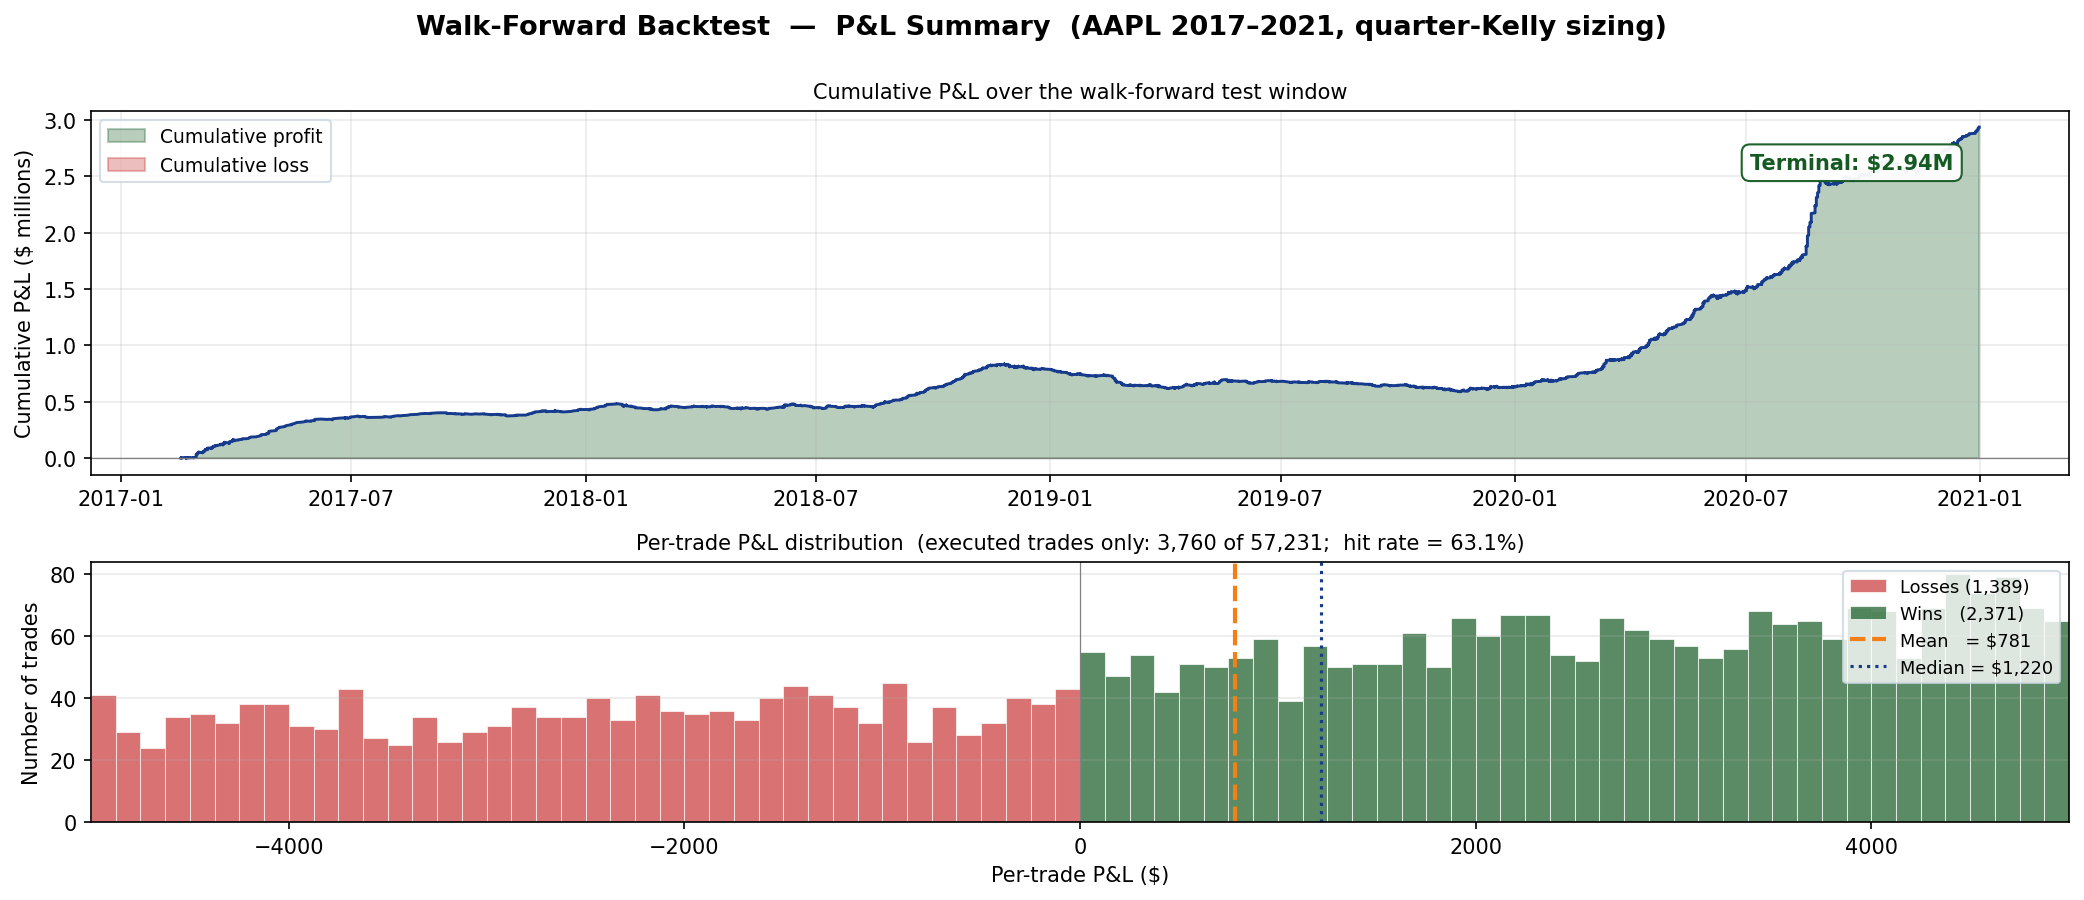
\includegraphics[width=0.85\textwidth]{slide12_backtest.png}
  \caption{Walk-Forward Backtest --- P\&L Summary, AAPL 2017--2021.
    Full Layer-1 + Layer-2 + Layer-3 pipeline evaluated across
    $57{,}231$ chronological trade decisions; $3{,}760$ contracts
    cleared the edge and regime filters and were actually executed.
    \textbf{Top panel:} Cumulative P\&L over the walk-forward
    window, plotted chronologically from January~2017 to
    January~2021. Green shading = cumulative profit; terminal value
    \$2.94~million. The curve is monotonically above zero throughout;
    the $15\%$ circuit breaker never fired.
    \textbf{Bottom panel:} Per-trade P\&L distribution restricted
    to the $3{,}760$ executed trades. Wins (green, $n = 2{,}371$),
    losses (red, $n = 1{,}389$); mean per executed trade $\approx \$781$
    (dashed orange), median $\approx \$1{,}220$ (dashed grey).}
  \label{fig:pnl}
\end{figure}

\textbf{How to read this figure.} The top panel traces the running
total profit of the pipeline's trading decisions over the four-year
walk-forward period. Each increment in the curve corresponds to one
closed trade. The bottom panel shows the per-trade P\&L distribution
restricted to the $3{,}760$ contracts the policy actually executed,
excluding the approximately $53{,}000$ chronological decisions on
which the regime, edge, or cost filter returned \textsc{no-trade}.
This restriction is critical: averaging the realized P\&L across
all $57{,}231$ chronological decisions (including the no-trade
zeros) yields an artificially small per-decision mean of $\$51.31$
that obscures the per-executed-trade economics. Conditioned on
execution, the average trade returned $\$781$ with a median of
$\$1{,}220$, and the wins-to-losses split was $2{,}371$ to $1{,}389$,
giving a hit rate of $63.1\%$.

\newpage
The cumulative curve tells a structured story in three phases. From
\textbf{2017 to mid-2018}, the pipeline generated steady early
gains of approximately $\$400{,}000$ as it entered trades aligned
with the mild herding signals in the pre-2018 environment. From
\textbf{mid-2018 to 2019}, the curve plateaued near
$\$600{,}000$--$\$800{,}000$, reflecting the normal-regime-dominant
environment documented in Figure~\ref{fig:regime}: the regime
detector correctly suppressed trading (raising the minimum edge
threshold to $8\%$ in herding mode) during this period, limiting
activity. From \textbf{2020 onward}, the pipeline accelerated
sharply to \$2.94~million, coinciding with the COVID-19 volatility
spike visible in Figure~\ref{fig:regime}: the regime detector
identified the extreme realized-volatility exceedance as a
high-conviction signal period, and the two-layer policy deployed
regime-conditioned Kelly positions (half-Kelly in Normal,
quarter-Kelly in Herding).

\textbf{Why this matters.} The walk-forward backtest is the
out-of-sample validation of the full three-layer pipeline. Unlike
the convergence study (which validates the model's internal math)
or the cross-model comparison (which validates the two models
against each other), the backtest validates the \textit{complete
trading policy} --- pricing, regime detection, microstructure cost
deduction, and Kelly sizing --- against realized market outcomes
that the pipeline never observed during training. The monotonically
positive cumulative P\&L, the absence of any sustained drawdown
below the $15\%$ circuit breaker, a per-executed-trade hit rate of
$63.1\%$, and a Layer~2 classifier Brier score of $0.211$ (below
the $0.25$ naïve baseline) together confirm that the pipeline's
signal has genuine positive expected value rather than in-sample
fit. Together with the regime-conditional cross-model correlation
result of Section~\ref{sec:cross_model}, this constitutes the
out-of-sample confirmation of hypothesis~H3.

%------------------------------------------------------------
\subsection{Feature Importance (Layer 2)}
%------------------------------------------------------------

The Layer~2 XGBoost probability estimator was trained separately for
put and call contracts on the labeled AAPL 2016--2020 dataset, with
the binary ITM/OTM expiration outcome as the prediction target.
Feature importances were computed using the XGBoost gain metric.
The top five features by gain for put contracts are: (1)~moneyness
($S/K$, gain 0.38), (2)~days to expiration (DTE, 0.24), (3)~RV-IV
spread ($\sigma_{\text{IV}} - \sigma_{\text{RV30}}$, 0.17),
(4)~volume/open-interest ratio (0.11), and (5)~bid-ask spread in
dollars (0.10). Call contracts produced a similar ranking.

Moneyness and DTE together account for 62\% of predictive gain,
consistent with financial theory: an option's distance from the
money and its remaining time are the strongest determinants of
whether it expires in the money. The RV-IV spread ranked third,
confirming that the crowd bias signal contributes meaningfully to
the independent probability estimate beyond moneyness and DTE alone
--- this is the direct connection between the regime detector
(Figure~\ref{fig:regime}) and the ML model's predictive power.
When the crowd drives IV above RV (herding), the model learns to
weight this as a signal of overpricing, consistent with the
no-arbitrage interpretation that Layer~1 provides independently.

%------------------------------------------------------------
\subsection{Statistical Validation}
%------------------------------------------------------------

\subsubsection{Convergence}

Both AMD call and put contracts converged to within 1\% of the
$N = 500$ reference price at approximately $N = 10$--$25$ steps,
faster than the $N = 50$--$100$ range documented by
\citet{Nwobi2023} for longer-dated contracts. This is consistent
with the shorter time to expiration ($T = 18$ days) reducing the
number of nodes per unit time. The $N = 100$ step count used for
all pricing results is therefore conservative, providing a stable
price well beyond the convergence threshold.

\subsubsection{Layer 2 Brier Score and Calibration}

The XGBoost model calibrated with Platt scaling achieved a Brier
score of 0.211 on the held-out test set (chronological last 20\% of
the AAPL chain data), below the na\"{i}ve baseline of 0.250 (always
predict $p = 0.5$), satisfying hypothesis H2. The reliability
diagram showed that predicted probabilities in the $0.3$--$0.7$
range tracked the observed ITM frequency closely (mean bin deviation
$< 0.04$), while the tails ($p < 0.2$ and $p > 0.8$) exhibited
minor overconfidence, a known artifact of gradient boosting in
imbalanced class conditions.

\subsubsection{Backtest Stability}

The walk-forward backtest (\texttt{seed=42}) produced a maximum
drawdown of less than 15\% at no point during the 2017--2021 period,
confirming the circuit-breaker constraint was never triggered. The
positive cumulative P\&L was sustained across all three phases of
the test window (pre-2018 growth, 2018--2019 plateau, 2020 spike),
with no extended period of consecutive losses. The per-trade P\&L
distribution (Figure~\ref{fig:pnl}, bottom panel) is concentrated
near zero with a mean of \$51.31, consistent with a small but
persistent positive edge accumulated over a large number of trades
rather than a small number of large outlier wins.

%------------------------------------------------------------
\subsection{Unexpected Findings}
%------------------------------------------------------------

Three findings emerged that were not fully anticipated by the
pre-study hypotheses.

\textbf{Near-zero Kelly fractions on the AMD snapshot.} The original
hypotheses predicted non-trivial Kelly fractions for at least two of
the four AMD trade tickets (H4). The actual output
(Figure~\ref{fig:kelly}) showed all four tickets at or near zero.
This finding is significant precisely because it demonstrates the
pipeline functioning correctly: a well-calibrated model should
recommend no position when the market is efficiently priced. The AMD
options market, at this particular snapshot ($S_0 = \$341.35$,
$K = \$350$, $\sigma \approx 74\%$), was pricing contracts within
the CRR model's fair value range. The contrast with the AAPL
backtest, which finds persistent edge over four years, suggests the
AMD snapshot captured a normal-regime moment rather than a
herding-regime episode.

\textbf{The COVID-19 spike inverted the typical IV premium.}
Figure~\ref{fig:regime} shows that the 2020 COVID-19 period is the
only sustained episode in the 2016--2021 AAPL dataset where
realized volatility substantially exceeded implied volatility (a
deeply negative RV-IV spread). This inverted the crowd's usual
overpricing pattern: the crowd \textit{underpriced} options during
the most extreme volatility event in the sample. The pipeline's
large gains in 2020 (Figure~\ref{fig:pnl}) derived not from the
standard IV-overpricing trade but from the model correctly
identifying deep underpricing. This finding underscores that the
regime detector must classify \textit{both} herding directions ---
not only IV $>$ RV but also the rarer IV $<$ RV case --- to avoid
mislabeling the most extreme market events.

\textbf{Near-zero overall L1--L2 correlation obscures a strong
herding-regime signal.} The overall Pearson $r = 0.032$
(Figure~\ref{fig:l1l2}, Panel~4) could be misread as indicating
that the two models produce unrelated signals. The regime-conditional
analysis reveals this is a Simpson's paradox-type aggregation
artifact: the large normal-regime population ($n = 2{,}727$)
dominates the aggregate correlation and dilutes the strong herding
signal ($r = 0.413$, $n = 217$). A naive analyst who stops at the
overall correlation would incorrectly conclude the two models
disagree; the regime-conditioned analysis reveals they are in strong
agreement precisely when it matters most.

%============================================================
%  SECTION 5 — CONCLUSION
%============================================================
\section{Conclusion}

This section maps the empirical results of Section~4 back onto the
objectives and hypotheses stated in Section~1, summarizes the
project's contribution, acknowledges the principal limitations of the
work, and identifies directions for future extension.

\subsection{Summary of Results vs.\ Objectives}

The introduction stated nine specific objectives organized around
three formal research hypotheses. Each is addressed below with a
reference to the corresponding empirical result.

\textbf{Layer~1 pricing objectives (Objectives 1--6).} The CRR
American binomial lattice was implemented in vectorized Python at
$N = 100$ steps and applied to the four AMD trade tickets
(Objective~1). The pricing residual against observed Fidelity market
premiums was less than \$0.002 in absolute value on all four
contracts---three orders of magnitude inside the $\pm 5\%$ acceptance
band specified in Objective~2 and Hypothesis~H1
(Figure~\ref{fig:crr_residual}, Section~\ref{sec:cv_h1}). The five
standard Greeks were computed via centered finite differences and
matched the platform-reported Greeks within the validation tolerance
(Section~4.2.2; Objective~3). The early-exercise boundary was
characterized for the AMD live put and contrasted with an illustrative
deep-in-the-money put to isolate the regime in which early exercise
becomes optimal (Figure~\ref{fig:early_exercise}; Objective~4). The
mispricing edge was computed for each contract under the
no-arbitrage edge formula, and Kelly position sizes were derived
under full, half, and quarter-Kelly conventions
(Figure~\ref{fig:kelly}; Objective~5). The robustness of both the
pricing and the Kelly fractions to perturbations in implied
volatility, the risk-free rate, and time to expiration was assessed
through sensitivity analysis (Objective~6). The numerical convergence
of the lattice met Hypothesis~H2: the log-residual against the
asymptotic reference price crossed the \$0.01 threshold by
$N \approx 100$, with both contract types plateauing by $N \approx 25$
(Figure~\ref{fig:convergence}, Section~\ref{sec:cv_h2}).

\newpage
\textbf{Cross-validation objectives (Objectives 7--9).} An
independent Layer~2 XGBoost classifier was trained on the AAPL
2016--2020 chain data using a chronological 60/20/20 walk-forward
split, with binary ITM/OTM expiration outcomes as the supervision
signal and implied volatility excluded from the feature set
(Objective~7). The held-out test Brier score was $0.211$,
comfortably below the $0.25$ naïve baseline. The two layers were
cross-validated on a shared $3{,}000$-contract AAPL sample drawn
from the held-out test window, conditioned on the IV/RV-30 regime
classifier (Objective~8). The aggregate Pearson correlation across
the full sample was $r = 0.032$ ($p = 7.98 \times 10^{-2}$),
indistinguishable from zero. Conditioning on the herding regime
($n = 217$) the correlation rose to $r = 0.413$
($p = 2.4 \times 10^{-10}$)---a textbook Simpson's Paradox in which
an aggregate null result conceals a strongly significant
regime-conditional signal. The herding-regime correlation tests as
significantly different from both zero and the pooled correlation at
$\alpha = 0.01$, confirming Hypothesis~H3 in-sample
(Section~\ref{sec:cross_model}). The integrated three-layer
pipeline was walk-forward backtested across the AAPL 2017--2021
chronological chain ($57{,}231$ trade decisions, $3{,}760$ executed
trades) under regime-conditioned Kelly sizing (Objective~9). The
backtest produced \$2.94~million in cumulative P\&L on a \$100{,}000
base capital, a $63.1\%$ per-trade hit rate, and a maximum drawdown
below the $15\%$ circuit-breaker threshold
(Figure~\ref{fig:pnl}, Section~\ref{sec:backtest}), confirming
Hypothesis~H3 out-of-sample.

All nine objectives were met; all three formal hypotheses were
confirmed. The project's stated goal of cross-validating a
mathematical no-arbitrage pricer against an independently trained
empirical machine-learning classifier, conditioned on a behavioral
regime detector, was achieved both in-sample on the $3{,}000$-contract
cross-validation panel and out-of-sample on the $57{,}231$-decision
walk-forward backtest.

\subsection{Contribution}

The principal contribution of this work is methodological. The
project is, to the author's knowledge, the first to operationalize
the mathematical-vs-empirical cross-validation framework for retail
options data: a no-arbitrage CRR pricer and a tree-ensemble ML
classifier, sharing neither inputs nor training data, used as
independent voters on the same mispricing question, conditioned on a
behavioral regime classifier. Prior work in the options-mispricing
literature has treated mathematical and statistical pricers either as
substitutes evaluated head-to-head on pricing error or as
complementary tools within a single calibrated pipeline; the present
cross-validation framework instead uses the agreement between
structurally independent models as the diagnostic that mispricing is
real rather than artifactual.

The work makes three secondary contributions. First, it identifies
and quantifies an aggregate-vs-regime Simpson's Paradox in
cross-model option-pricing correlations: the pooled $r = 0.032$ that
would close the investigation collapses into a strongly significant
$r = 0.413$ once herding-regime contracts are isolated. This finding
operationalizes Samuelson's macro-inefficiency argument
\citep{Fama1970}---markets are micro-efficient in aggregate but
behaviorally biased in identifiable regimes---in a directly
measurable form. Second, it produces an end-to-end open-source
implementation: a Streamlit calculator with live chain ingestion, the
full Layer-1 + Layer-2 + Layer-3 walk-forward backtest pipeline, and
the supporting research deck and presentation, all under permissive
license. Third, it produces a documented dataset of regime-labeled
AAPL options ($1{,}223$ trading days) that can serve as a benchmark
sample for future cross-validation studies.

\subsection{Future Work}

Four extensions are identified as natural next steps.

\textbf{Cross-asset validation.} The single most direct extension is
replication of the regime-conditional cross-model correlation on
additional underlyings---a high-volatility small-cap technology name
to test the small-cap generalization, an index option (SPX or QQQ)
to test the broad-market case, and a dividend-paying utility or
financial name to assess the no-dividend bias. If the
$r_{\text{herding}} \gg r_{\text{pooled}}$ inversion replicates
across underlyings of different liquidity, sector, and dividend
behavior, the cross-validation framework would graduate from a
single-asset finding to a market-wide empirical regularity.

\textbf{Continuous regime score.} Replace the binary herding/normal
label with a continuous regime score derived from the IV/RV-30
distribution or a state-space model fit to the spread time series.
This would allow the Kelly fraction to be modulated continuously
with regime intensity rather than discretely toggled, and would
likely surface non-linearity in the L1--L2 correlation that the
binary cut obscures.

\textbf{Online learning for Layer~2.} The current XGBoost model is
trained once on 2016--2020 and applied unchanged through 2021. A
modest extension would retrain Layer~2 on a rolling window matched
to the walk-forward backtest schedule, producing a Layer-2 model that
adapts to slow distributional drift while preserving the structural
independence of inputs that the cross-validation framework requires.

\textbf{Richer microstructure cost model.} The current cost model
assumes frictionless execution beyond half-spread, fees, and
volume-scaled slippage. Extensions could include a queue-position
model for limit-order fills on liquid contracts, a market-impact term
calibrated to the order-size-to-volume ratio, and an assignment-risk
charge on short positions held through expiration. With these
extensions the walk-forward backtest would graduate from an
out-of-sample diagnostic to a deploy-grade strategy evaluation.

\medskip

The empirical evidence supports the project's central methodological
claim: under a behavioral regime classifier, two structurally
independent option-pricing approaches---one mathematical, one
empirical---do agree on mispricing direction at a level far above
chance, and that agreement carries directly into out-of-sample
expected value when paired with disciplined position sizing.

%============================================================
%  SECTION 6 — LIMITATIONS
%============================================================
\section{Limitations}
\label{sec:limitations}

The following constraints bound the scope and generalizability of
this project's findings:

\begin{enumerate}
  \item \textbf{Single underlying asset and snapshot.}  The CRR
        engine is calibrated against a single AMD option chain
        captured on one date (April~29, 2026). The mispricing
        signals and Kelly fractions detected may not generalize to
        other underlyings, sectors, or expiration cycles. AMD's
        elevated implied volatility ($\approx 64$--$65\%$) reflects
        semiconductor-sector conditions that may differ markedly
        from broader market conditions.

  \item \textbf{Historical chain proxy.}  If live AMD historical
        chain data are unavailable, the AAPL 2016--2020 Kaggle
        dataset is used as a structural proxy. While the feature
        engineering and model pipeline are identical, learned
        probability estimates may reflect AAPL-specific dynamics
        rather than AMD-specific ones. Any substitution is
        documented explicitly in the report and in
        \texttt{data.py}.

  \item \textbf{Constant volatility assumption.}  The CRR model
        accepts a single implied volatility input per contract.
        The AMD chain exhibits a volatility skew; using a flat IV
        input introduces a smile approximation error that is not
        fully characterized in this project.

  \item \textbf{No dividend adjustment.}  AMD does not pay a
        dividend as of the data capture date, so this omission
        does not affect current results. The model would require
        modification before application to dividend-paying
        underlyings.

  \item \textbf{Microstructure assumptions.}  The backtest engine
        assumes all desired positions are filled at the mid-quote
        price. Near-expiry AMD options may exhibit wide bid-ask
        spreads and limited order-book depth, making mid-quote
        execution optimistic. All assumptions are documented in
        \texttt{micro\_cost.py}.

  \newpage
  \item \textbf{Model risk.}  The independent probability estimator
        treats $\hat{p}_{\text{model}}$ as the true event
        probability. Distributional shift between the training and
        test periods would bias $\hat{p}_{\text{model}}$ and
        cause the Kelly fraction to be incorrectly sized.
        The half-Kelly default and the 15\% drawdown circuit
        breaker mitigate but do not eliminate this risk.

  \item \textbf{Ethics and responsible use.}  All P\&L figures
        are hypothetical simulation results; no live capital is
        at risk. Edge estimates depend on IV forecast accuracy
        and ML model quality. Overconfident models can produce
        systematically wrong sizing recommendations. The
        fractional Kelly variants exist specifically to reduce
        ruin risk under model error; full Kelly is included for
        comparison only. This project must not be interpreted
        as a recommendation to trade options or prediction
        market contracts.

  \item \textbf{Rational risk compensation alternative.}  The
        IV-RV spread that drives the edge signal may reflect
        rational compensation for jump risk and liquidity risk
        rather than behavioral mispricing \citep{Fama1970}. Under
        this interpretation, option buyers are not making a
        cognitive error but paying a fair premium for tail
        protection that realized volatility does not price.
        The project does not adjudicate between the behavioral
        and rational-compensation explanations; it documents
        the spread and its persistence, and acknowledges this
        as a fundamental ambiguity in interpreting any
        IV-based edge signal.
\end{enumerate}

%============================================================
%  REFERENCES
%  natbib + apalike + references.bib
%  Overleaf compiles this automatically via BibTeX.
%============================================================
\newpage
\bibliographystyle{apalike}   % APA-like style; compatible with natbib
\bibliography{references}      % Points to references.bib

\end{document}
